\documentclass[14pt]{extarticle}
\usepackage[utf8]{inputenc}
\usepackage{amsmath}
\usepackage{amsfonts}
\usepackage{graphicx}
\usepackage{setspace}
\usepackage{geometry}
\usepackage{enumitem}
\usepackage{amssymb}
\usepackage{xcolor}
\usepackage{mathtools}
\usepackage{float}
\usepackage{listings} % Added to define the 'lstlisting' environment


\geometry{
    top=1in,
    bottom=1in,
    left=1in,
    right=1in,
    headheight=14pt,
    headsep=25pt,
    footskip=30pt
}

\title{Bayes Theorem}
\author{Yana Jin}
\date{Wednesday, 11th September 2024}

\onehalfspacing

% Create a new command for the cover page
\newcommand{\coverpage}{%
    \begin{titlepage}
        \centering
        
\includegraphics[width=1\textwidth]{cover.png}
    \end{titlepage}
}

\begin{document}

% Insert the cover page
\coverpage

% Start a new page for the content
\newpage

\section*{Tests Based on Population Models}

Getting null distribution based on randomization can be difficult if:

\begin{itemize}
    \item experiment is complicated
    \item experiment is non or partially randomized
    \item experiment includes nuisance factors
\end{itemize}

\noindent Consider the following model for our 2 treatment experiment:

\begin{itemize}
    \item There is a large/infinite population of similar individuals as those in our experiment.
    
    \item When treatment A is given, the distribution of outcomes can be represented by probability distribution \( p_A \):
    \[
    \mathbb{E}(Y_A) = \int y p_A(y) \, dy = \mu_A
    \]
    \[
    \text{var}(Y_A) = \mathbb{E} [ (Y_A - \mu_A)^2 ] = \sigma_A^2
    \]
    
    \item When treatment B is given, we have probability distribution \( p_B \):
    \[
    \mathbb{E}(Y_B) = \mu_B
    \]
    \[
    \text{var}(Y_B) = \sigma_B^2
    \]
    
    \item The individuals that got treatment A in our experiment can be viewed as an independent sample from \( P_A \).
    
    \item Similarly for those receiving treatment B.
    
    \[
    Y_{1A}, \dots, Y_{n_A A} \sim P_A
    \]
    \[
    Y_{1B}, \dots, Y_{n_B B} \sim P_B
    \] 
\end{itemize}

\textbf{Recall}
\[
\mathbb{E} \left( \bar{Y}_A \right) = \mathbb{E} \left( \frac{1}{n_A} \sum_{i=1}^{n_A} Y_{iA} \right) = \frac{1}{n_A} \sum_{i=1}^{n_A} \mu_A = \mu_A
\]
\[
\text{var} \left( \bar{Y}_A \right) = \text{var} \left( \frac{1}{n_A} \sum_{i=1}^{n_A} Y_{iA} \right) = \frac{1}{n_A^2} \sum_{i=1}^{n_A} \sigma_A^2 = \frac{\sigma_A^2}{n_A}
\]
\[
\therefore\ \text{as } n_A \to \infty, \quad 
\text{var} \left( \bar{Y}_A \right) \to 0
\]
\[
\text{and together with unbiasedness, }
\bar{Y}_A \to \mu_A \quad \textcolor{red}{\text{(consistent estimator)}}
\]

\textbf{Can also show}
\[
S_A^2 \to \sigma_A^2
\]
\[
\frac{\# \left\{ Y_{iA} \leq x \right\}}{n_A} = \hat{F}_A(x) \to F_A(x) = \int_{-\infty}^x p_A(y) dy
\]

\section*{Connection to Hypothesis Testing}
We can then formulate \( H_0 \) and \( H_1 \) in terms of population quantities:
\[
H_0: \mu_A = \mu_B
\]
\[
H_1: \mu_A \neq \mu_B
\]

\textbf{Assume:}
\[
Y_{1A}, \dots, Y_{n_A A} \sim P_A
\]
\[
Y_{1B}, \dots, Y_{n_B B} \sim P_B
\]

\textbf{The null hypothesis \( H_0 \) can be re-expressed as:}
\[
\int y p_A(y) \, dy = \int y p_B(y) \, dy
\]

To evaluate and get a p-value, we need the distribution of \( g(Y_A, Y_B) \) under \( \mu_A = \mu_B \). 
\textcolor{red}{This involves assumptions about \( P_A \) and \( P_B \).}

\section*{The Normal Distribution}

\begin{figure}[h]
    \centering
    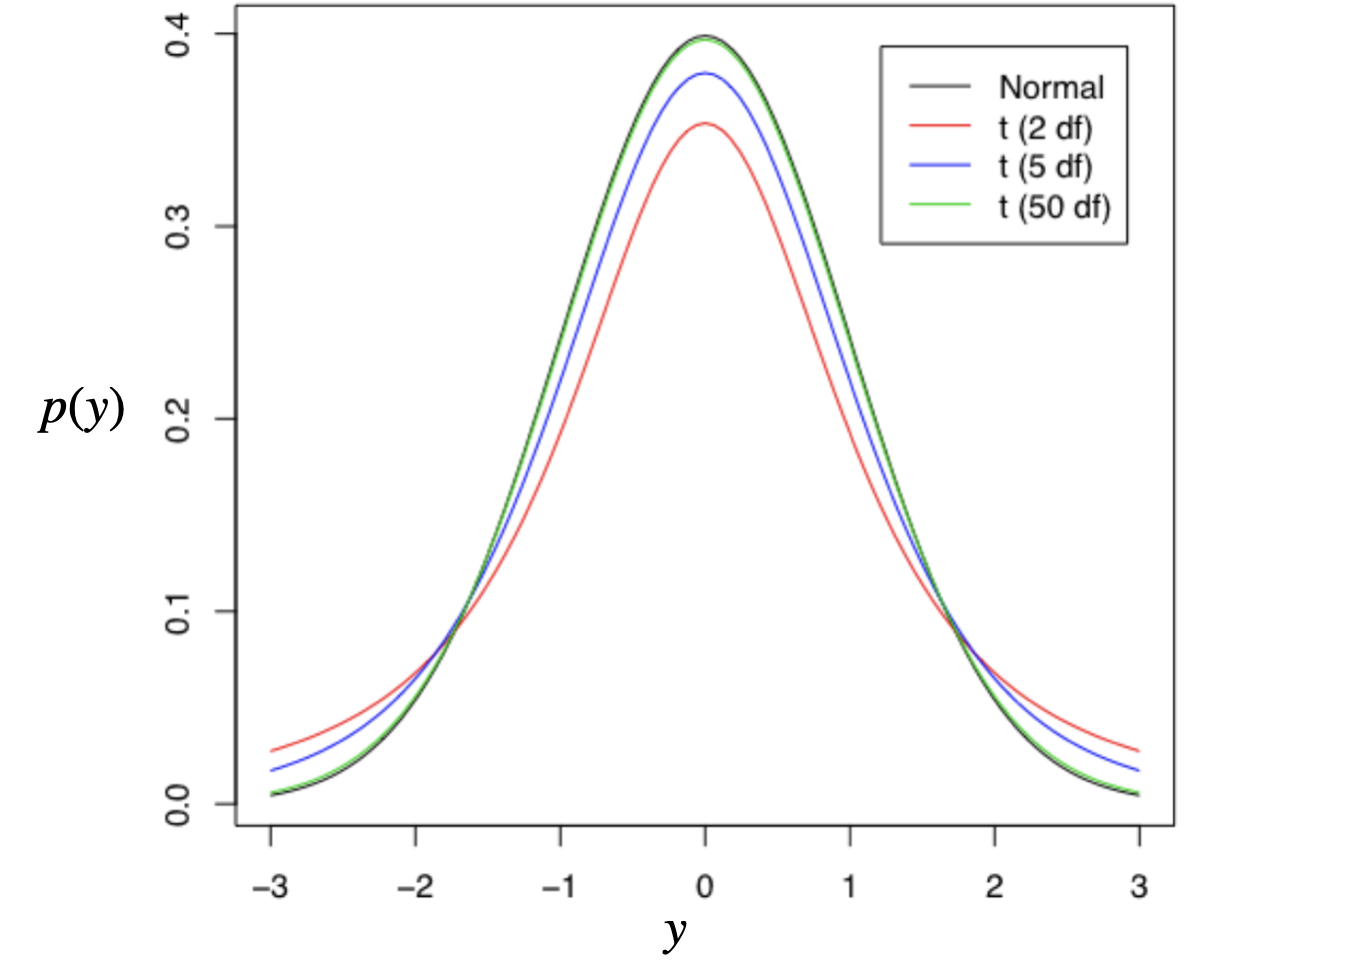
\includegraphics[width=0.75\textwidth]{fig1.png}
\end{figure}

Why is this a useful assumption to make?

\begin{itemize}
    \item Data can be (approximately) normally distributed.
    \item Sample means are (approximately) normally distributed.
\end{itemize}

Both due to \textcolor{blue}{Central Limit Theorem}. 

Let \( P(\mu, \sigma^2) \) denote a population with mean \( \mu \) and variance \( \sigma^2 \). Then,

\[
\left.
\begin{array}{l}
Y_1 \sim P_1(\mu_1, \sigma_1^2) \\
Y_2 \sim P_2(\mu_2, \sigma_2^2) \\
\vdots \\
Y_m \sim P_m(\mu_m, \sigma_m^2)
\end{array}
\right\}
\Rightarrow \sum_{j=1}^{m} Y_j \overset{\cdot}{\sim} \mathcal{N} \left( \sum_{j=1}^{m} \mu_j, \sum_{j=1}^{m} \sigma_j^2 \right)
\]
\[\quad \textcolor{red}{\text{(if the $Y_j$'s are independent)}}
\]

\textcolor{blue}{Sums of varying quantities are approximately normally distributed.}

\section*{Normally Distributed Data}
Consider:
\[
Y_i = \beta_1 X_1 + \beta_2 X_2 + \beta_3 X_3 + \dots
\]
Empirical distribution of \( Y_i \)'s will be approximately \( N(\mu, \sigma^2) \) where \( \mu \) and \( \sigma^2 \) depend on \( \beta_1, \beta_2, \dots \), and the means and variances of \( X_1, X_2, X_3, \dots \).

\textcolor{blue}{Additive effects \( \Rightarrow \) approx normally distributed data.}

\section*{Normally Distributed Means}
For experiment 1:
\[
\text{sample: } y_1^{(1)}, \dots, y_n^{(1)} \text{ i.i.d.} \, P \Rightarrow \bar{y}^{(1)}
\]
\[\vdots\]
For experiment \( m \):
\[
\text{sample: } y_1^{(m)}, \dots, y_n^{(m)} \text{ i.i.d.} \, P \Rightarrow \bar{y}^{(m)}
\]
A histogram of \( \{ \bar{y}^{(1)}, \dots, \bar{y}^{(m)} \} \) will be approx \( N(\mu, \sigma^2/n) \).

\textcolor{blue}{This is the sampling distribution of the sample mean even if the original data are not normal.}

\section*{Basic Properties of the Normal Distribution}
- If \( Y \sim N(\mu, \sigma^2) \), then \( a Y + b \sim N(a \mu + b, a^2 \sigma^2) \) for some constants \( a \), \( b \). \\ 
- If \( Y_1 \sim N(\mu_1, \sigma_1^2) \), \( Y_2 \sim N(\mu_2, \sigma_2^2) \), and \( Y_1, Y_2 \) are independent:
\[
\Rightarrow Y_1 + Y_2 \sim N(\mu_1 + \mu_2, \sigma_1^2 + \sigma_2^2)
\]
- If \( Y_1, \dots, Y_n \) are i.i.d. \( N(\mu, \sigma^2) \), then \( \bar{Y} \) is independent of \( S^2 \) \textcolor{blue}{ (sample variance)}.

\noindent \textbf{How does this help with hypothesis testing?}

Consider:
\[
H_0: \mu_A = \mu_B
\]

Under \( H_0 \):
\[
\bar{Y}_A \overset{\cdot}{\sim} N(\mu, \sigma_A^2 / n_A)
\]
\[
\bar{Y}_B \overset{\cdot}{\sim} N(\mu, \sigma_B^2 / n_B)
\]
\[
\bar{Y}_B - \bar{Y}_A \overset{\cdot}{\sim} N(0, \sigma_{AB}^2)
\]

Where:
\[
\sigma_{AB}^2 = \frac{\sigma_A^2}{n_A} + \frac{\sigma_B^2}{n_B}
\]
\[
\textcolor{blue}{\Rightarrow \therefore \text{ if know variances, would have a null sampling distribution.}}
\]

\newpage

\noindent \textcolor{red}{\textbf{History of the Neyman-Pearson Approach and the p-Value Approach}}

\begin{figure}[h]
    \centering
    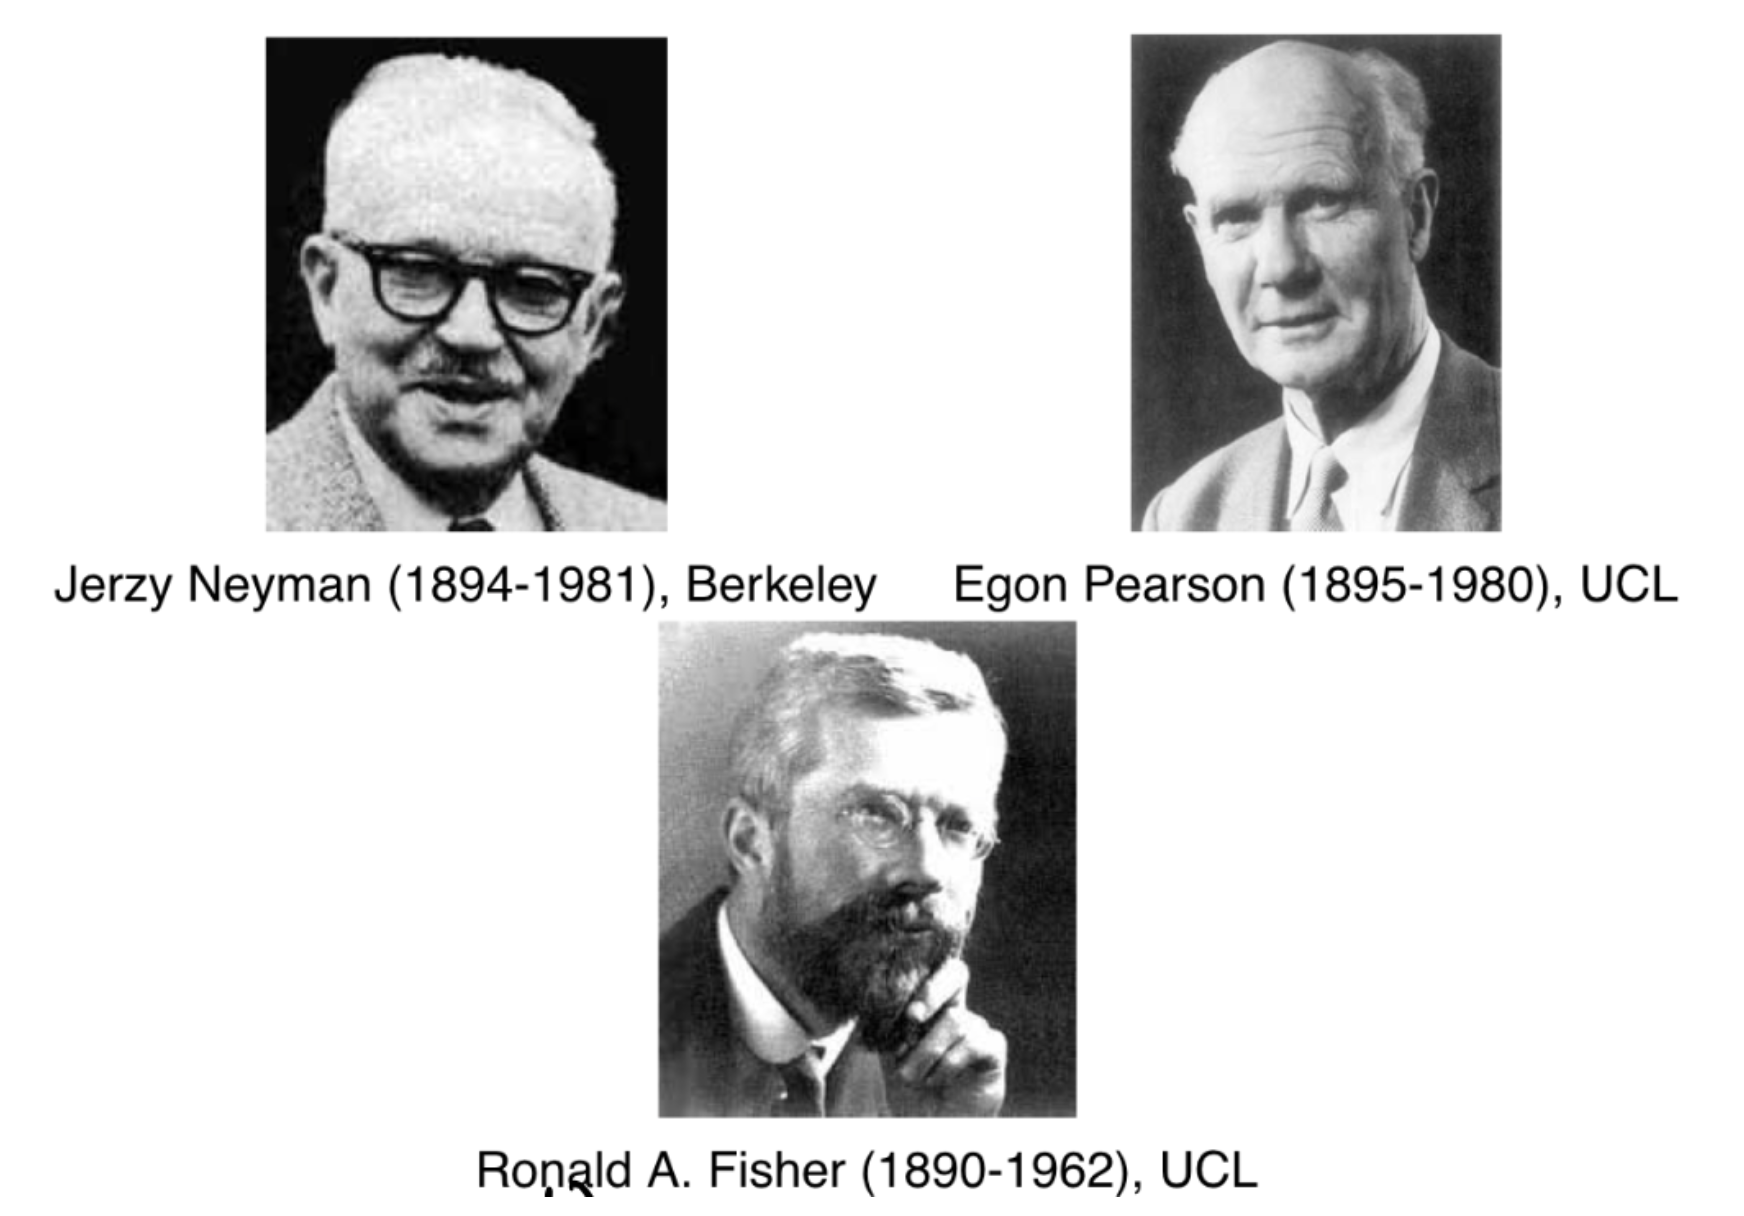
\includegraphics[width=1\textwidth]{fig2.png}
\end{figure}

The rejection/\textcolor{red}{do not reject} dichotomy is associated with the Neyman-Pearson approach to hypothesis testing; p-value is associated with R.A. Fisher.

\newpage

\section*{The t-test (One-sample) }
Let's consider first a simple one sample hypothesis test:
\[
Y_1, \dots, Y_n \sim \text{ i.i.d.  with mean } \mu \text{ and variance } \sigma^2
\]
\[
H_0: \mu = \mu_0
\]
\[
H_1: \mu \neq \mu_0
\]
\textcolor{blue}{Example: 
\[
Y_i = \text{muscle strength after treatment} - \text{muscle strength before treatment}
\]
\[
H_0: \mathbb{E}(Y_i) = \mu = 0
\]}

\begin{figure}[h]
    \centering
    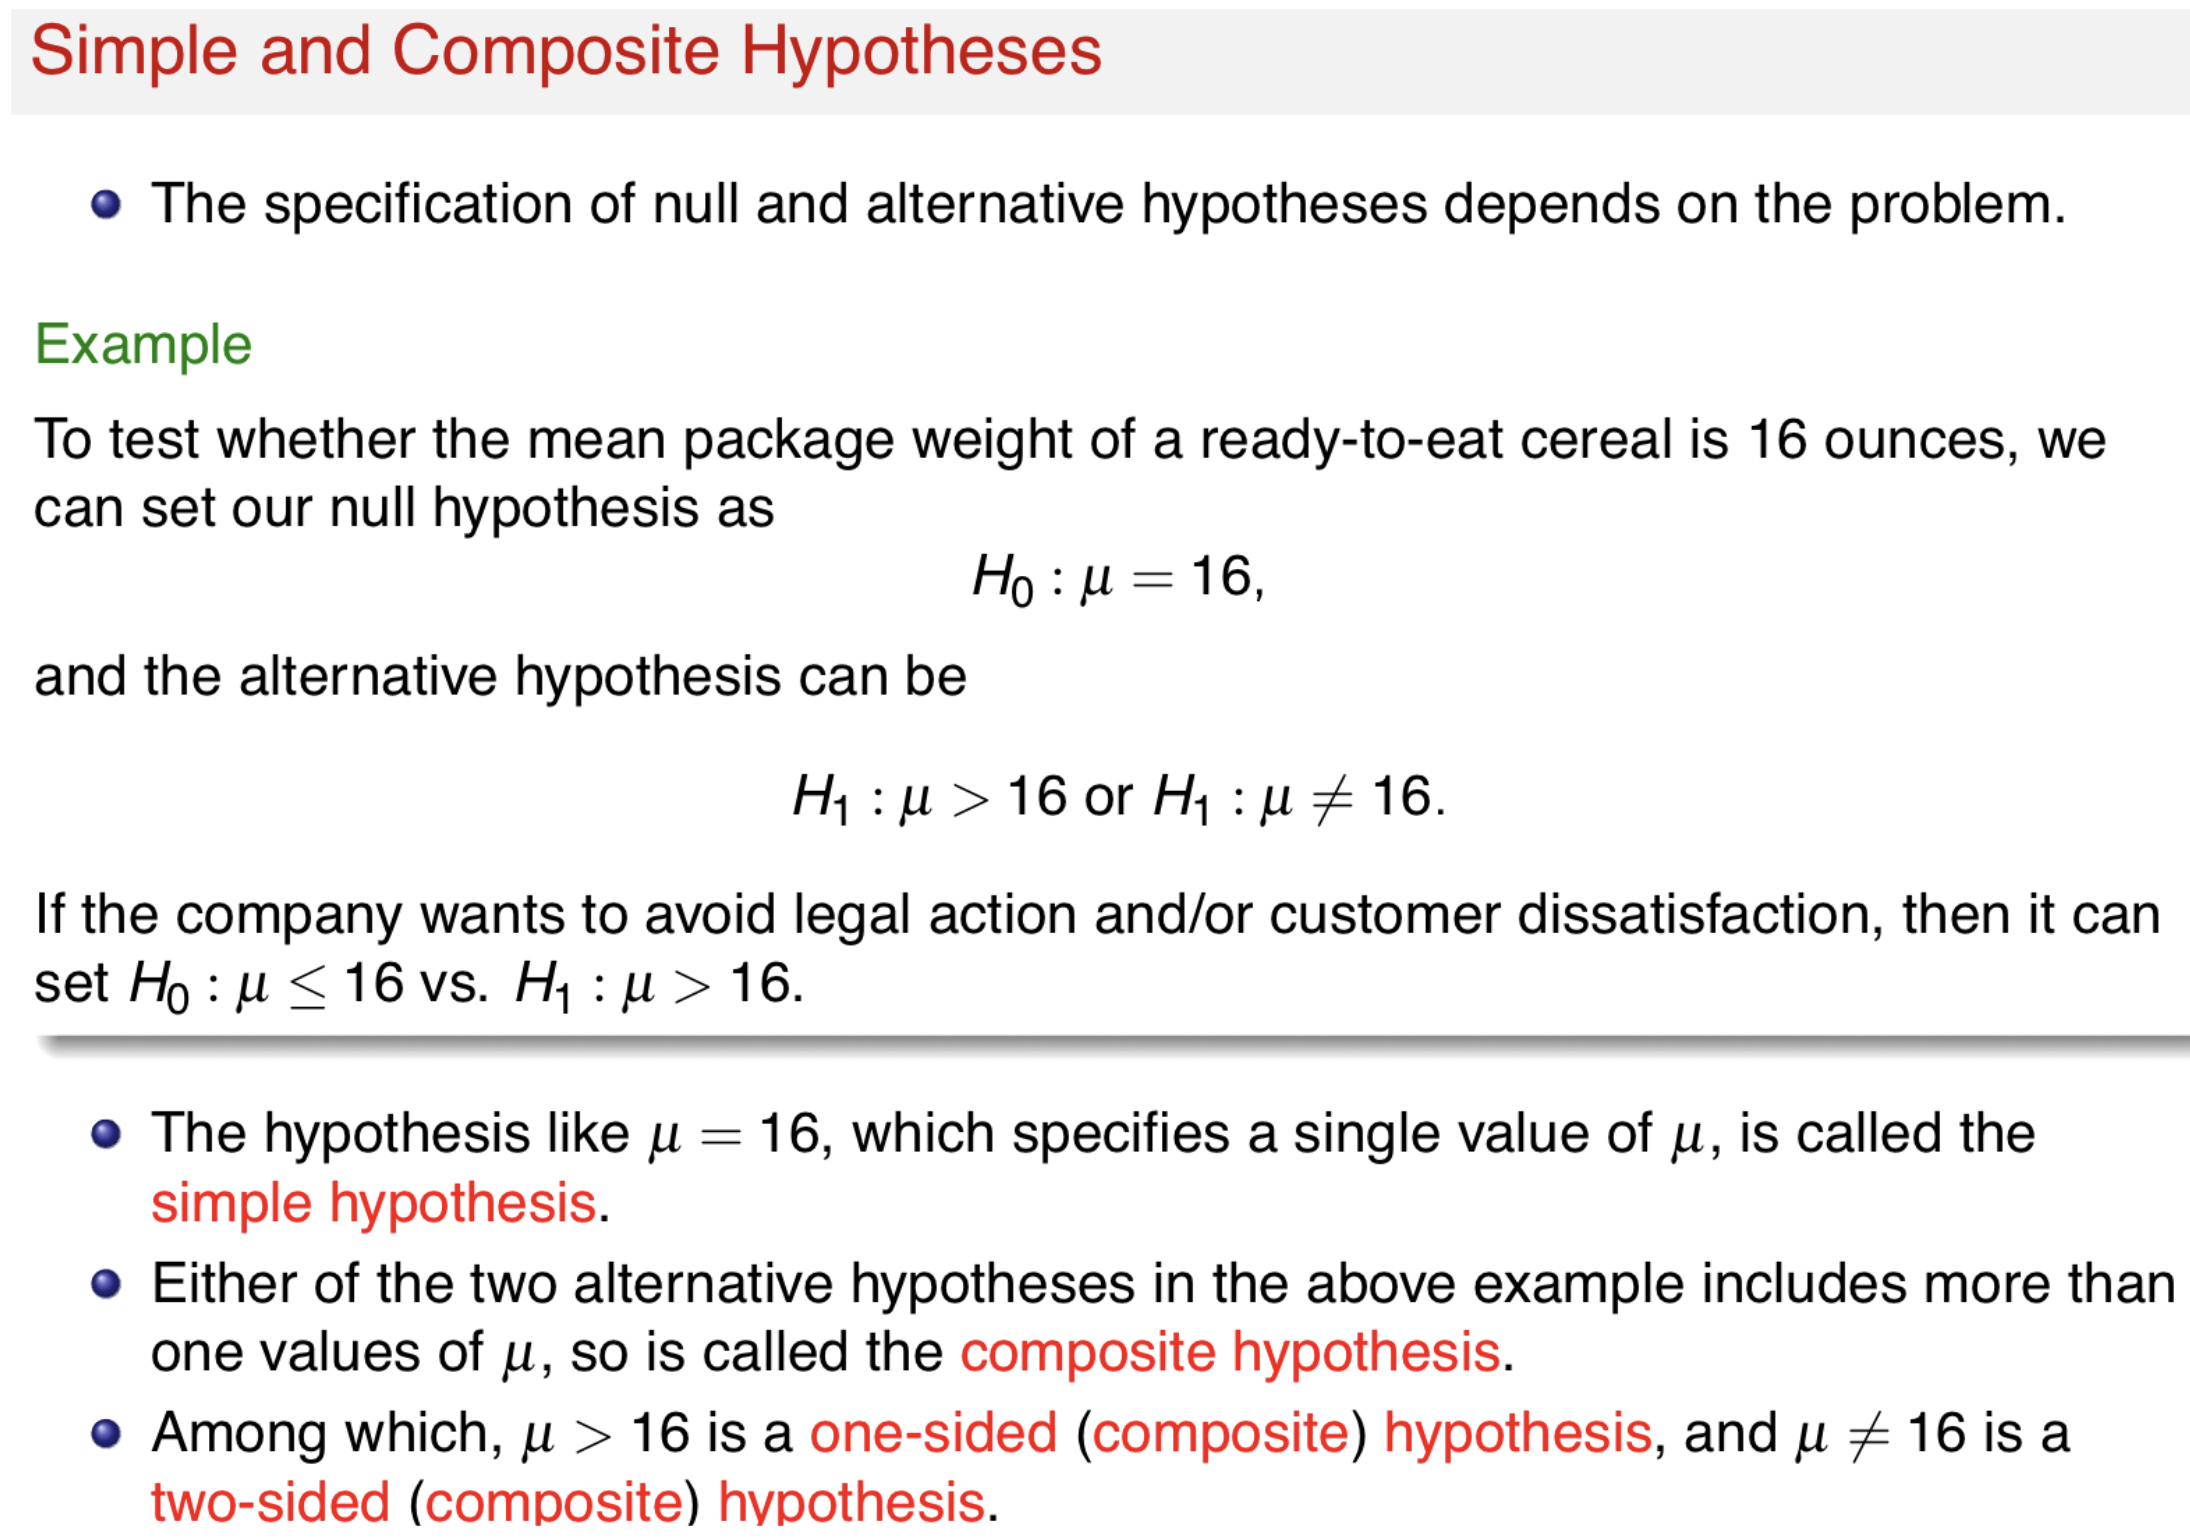
\includegraphics[width=1\textwidth]{fig3.png}
\end{figure}

\vspace{1cm}

\textbf{Consider: } 

$\left| \bar{Y} - \mu_0 \right|$ \text{ as a test statistic}

- sensitive to deviations from $H_0$ 

- sampling distribution approximately known

\[
\mathbb{E}(\bar{Y}) = \mu
\]
\[
\text{var}(\bar{Y}) = \frac{\sigma^2}{n}
\]
\[
\bar{Y} \approx \text{normal}
\]

$\therefore$ Under $H_0$,
\[
\left( \bar{Y} - \mu_0 \right) \overset{\cdot}{\sim} N \left( 0, \frac{\sigma^2}{n} \right)
\]
\[\quad \text{but} \quad \sigma^2 \text{ is unknown}\]

What if we scale $\left( \overline{Y} - \mu_0 \right)$?
\[
\Rightarrow \frac{\overline{Y} - \mu_0}{\textcolor{red}{\frac{\sigma}{\sqrt{n}}}} \sim N(0,1) \ \text{under} \ H_0
\]
\[
\textcolor{red}{\text{where} \ \ SE = \sqrt{\text{var}} }
\]

Having observed data,

$\quad \overline{Y} \text{ is computable}, $

$\quad n \text{ is known}, $

$\quad \mu_0 \text{ is hypothesized (known)}, $

$\quad \sigma \text{ is unknown} $

Solution: plug in $s^2$ for $\sigma^2$

\section*{One Sample t-statistic}
For random variable $Y$, the test statistic is:
\[
t(Y) = \frac{\bar{Y} - \mu_0}{s / \sqrt{n}}
\]

\noindent \textbf{What is the null distribution for} \(t(\mathbf{y})\)?

\noindent If approximation \(s^2 \approx \sigma^2\) is poor, then we need to take into account uncertainty in our estimate of \(\sigma^2\).\\
\noindent\textcolor{blue}{This can happen for instance with small n.}


\section*{Some Facts}
- If \( Z_1, \dots, Z_n \sim i.i.d \quad N(0,1) \),
\[
\Rightarrow \sum_{i=1}^n Z_i^2 \sim \chi_n^2
\]
\[also \quad
\Rightarrow \sum_{i=1}^n (Z_i - \bar{Z})^2 \sim \chi_{n-1}^2
\]

- If $Y_1, \dots, Y_n \quad \text{i.i.d.  } {\sim} \quad \mathcal{N}(\mu, \sigma^2)$
\[
\Rightarrow \frac{Y_1 - \mu}{\sigma}, \dots, \frac{Y_n - \mu}{\sigma} \quad \text{i.i.d.  } {\sim} \quad \mathcal{N}(0,1)
\]
\[
\Rightarrow \frac{1}{\sigma^2} \sum_{i=1}^{n} (Y_i - \mu)^2 \sim \chi_n^2 \\
\]
\[
\text{Also}
\Rightarrow \frac{1}{\sigma^2} \sum_{i=1}^{n} (Y_i - \overline{Y})^2 \sim \chi_{n-1}^2
\]
\begin{figure}[h]
    \centering
    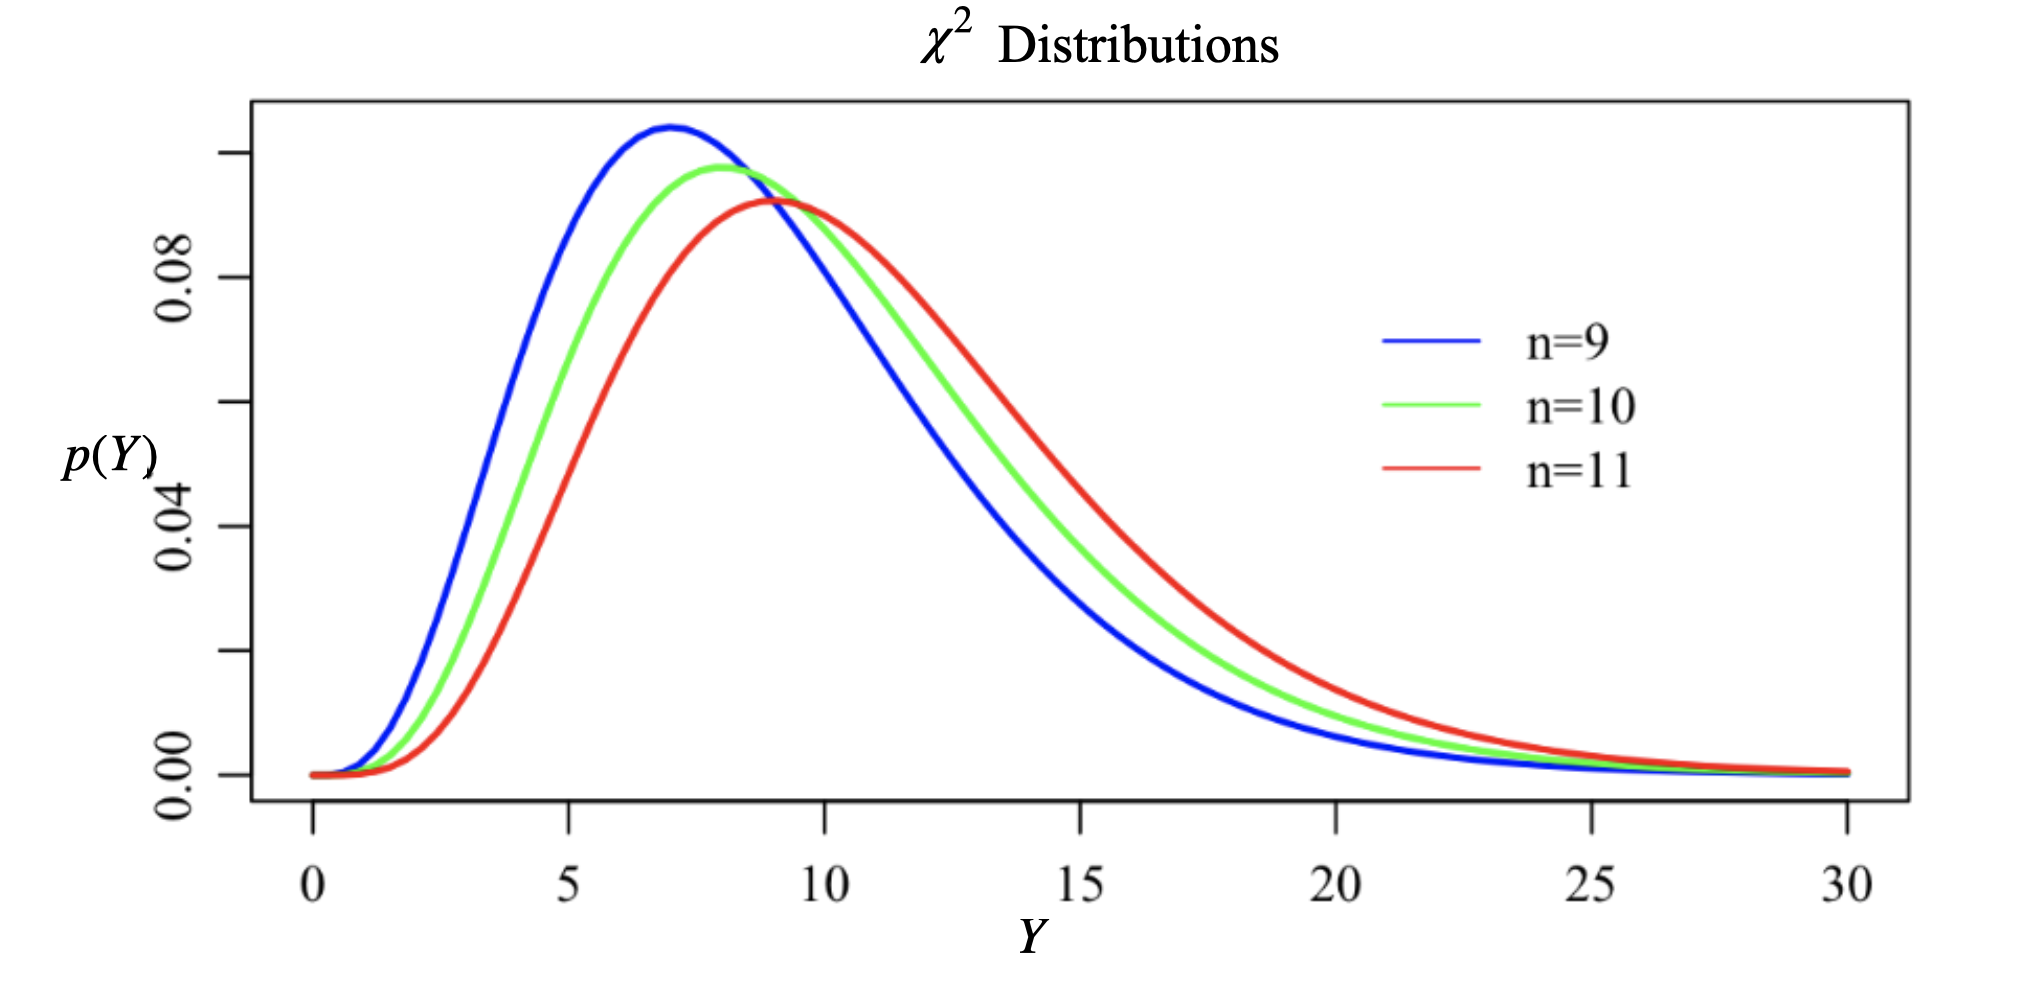
\includegraphics[width=1\textwidth]{fig4.png}
\end{figure}

So all of this allows us to do: 
\[
\frac{n-1}{\sigma^2} s^2 = \left(\frac{n-1}{\sigma^2}\right) \left( \frac{1}{n-1} \sum_{i=1}^n (Y_i - \bar{Y})^2 \right) \sim \chi^2_{n-1}
\]

\section*{The t-distribution}
If:
\[
Z \sim N(0, 1), \quad X \sim \chi^2_m, \quad Z \text{ and } X \text{ are independent,}
\]
\[
\Rightarrow \frac{Z}{\sqrt{X/m}} \sim t_m
\]
See more examples below.
\newpage

\begin{figure}[h]
    \centering
    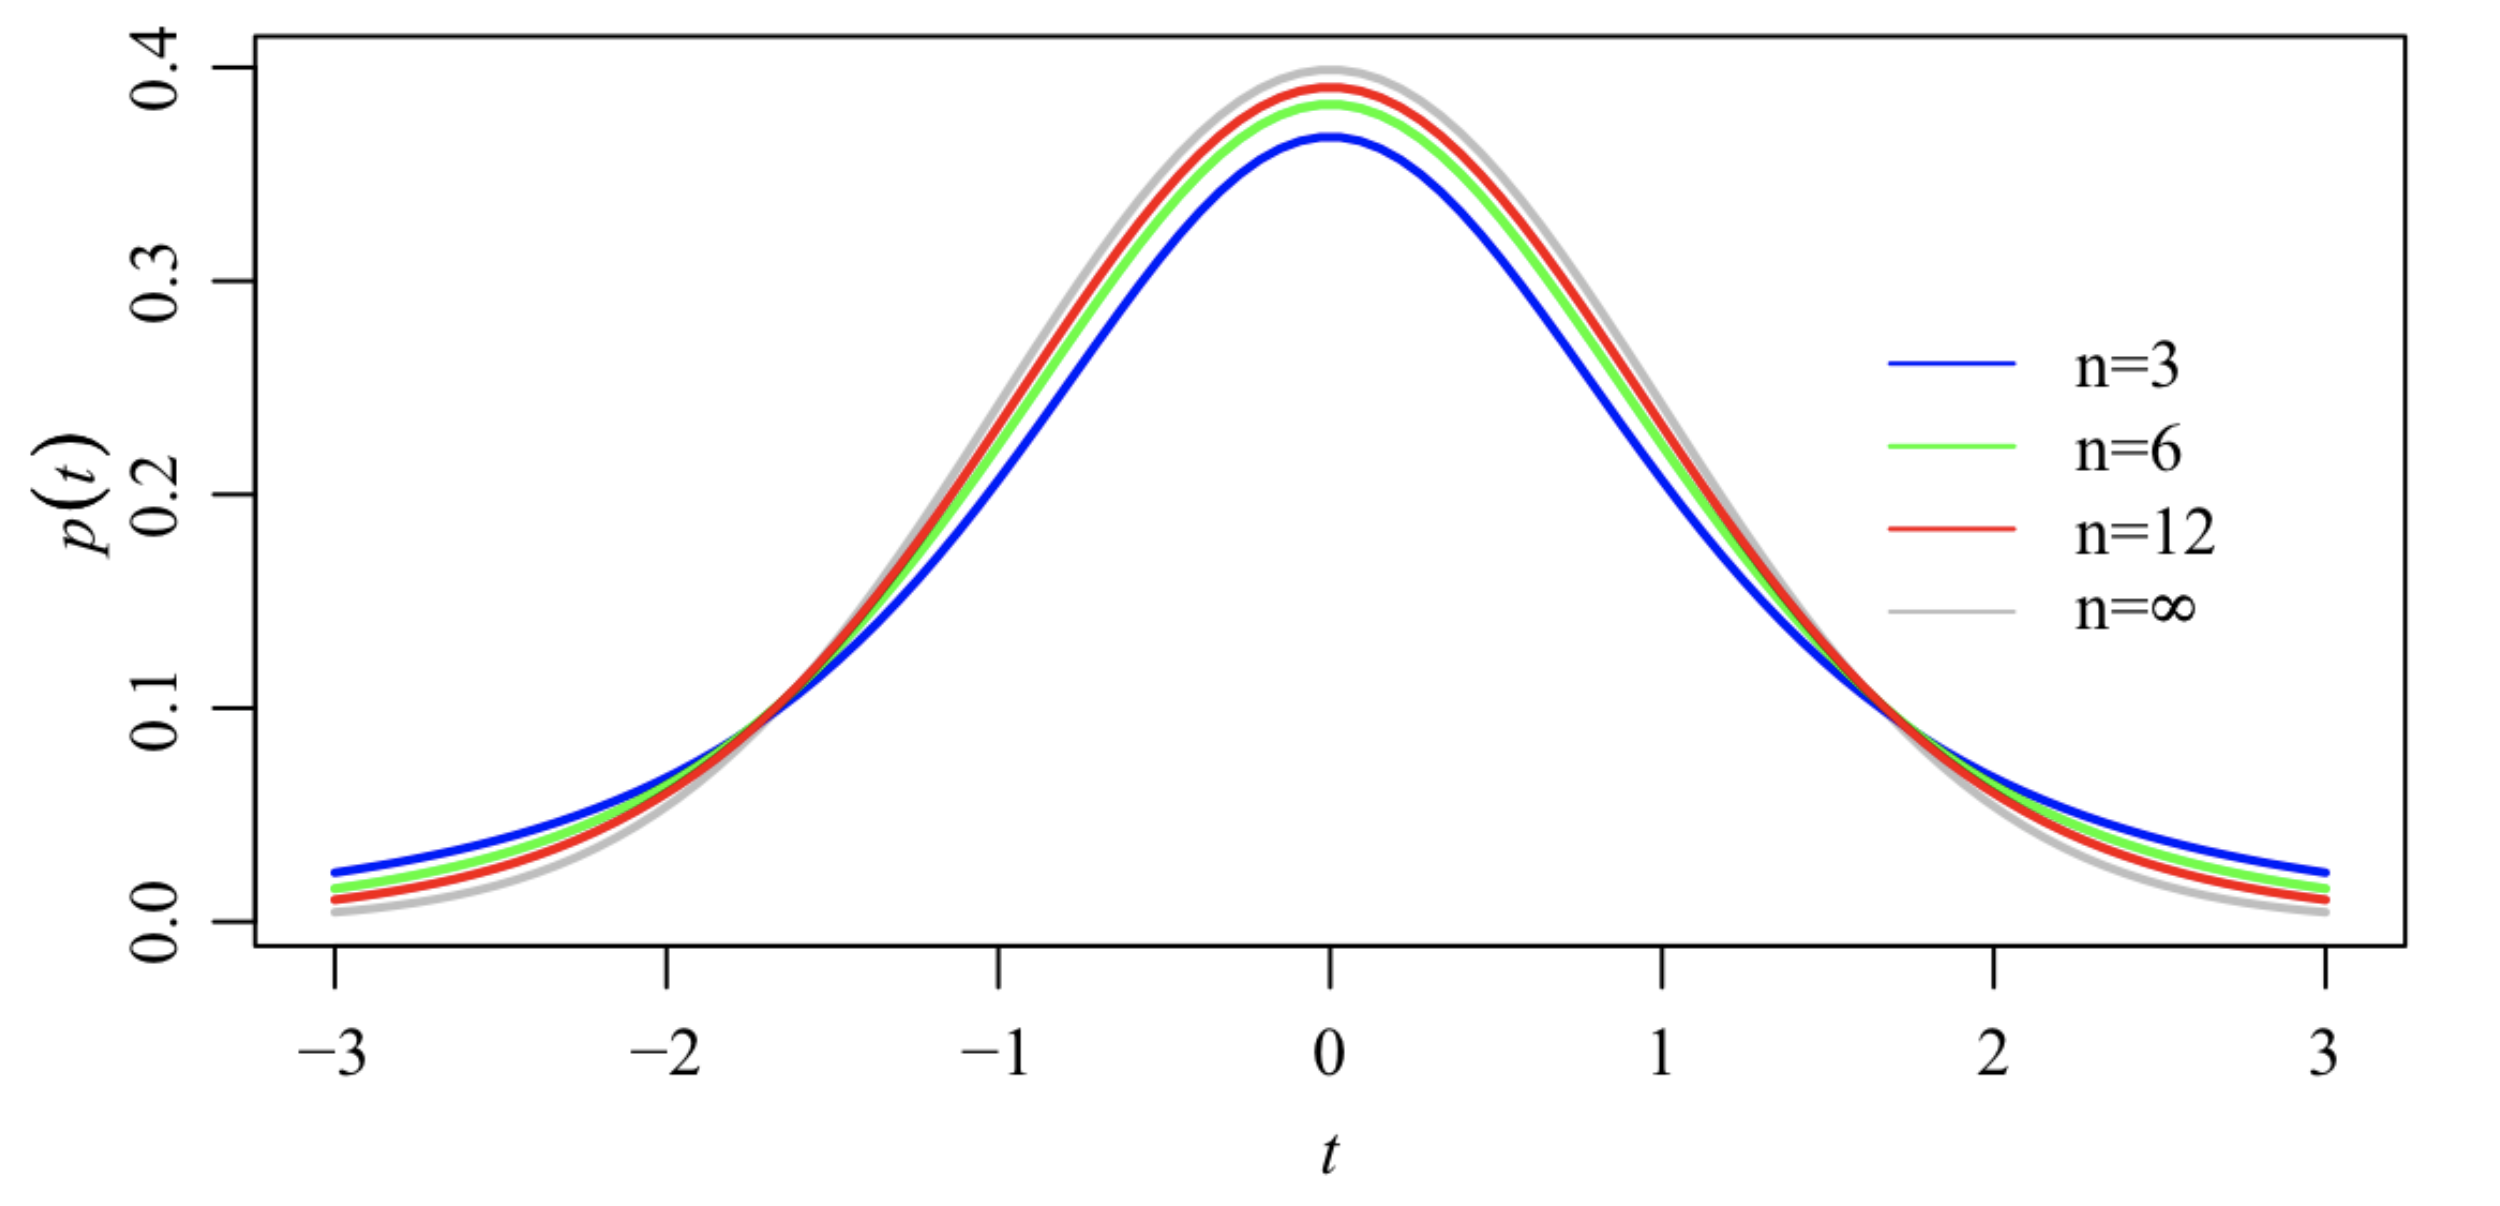
\includegraphics[width=1\textwidth]{fig5.png}
\end{figure}
\text{How does this help?}
\[
\frac{\sqrt{n} \left( \bar{Y} - \mu \right)}{\sigma} \sim \mathcal{N}(0, 1)
\]
\[
\frac{n-1}{\sigma^2} s^2 \sim \chi^2_{n-1}
\]
\[
\bar{Y} \text{ and } s^2 \text{ are independent}
\]

Let
\[
Z = \frac{\sqrt{n} \left( \overline{Y} - \mu \right)}{\sigma}
\]
\[
X = \frac{n - 1}{\sigma^2} s^2
\]

Then, 
\[
\frac{Z}{\sqrt{\frac{X}{n-1}}} = \frac{\frac{\sqrt{n} \left( \overline{Y} - \mu \right)}{\sigma}}{\sqrt{\frac{\frac{n-1}{\sigma^2} s^2}{n-1}}} = \frac{\overline{Y} - \mu}{\frac{s}{\sqrt{n}}} \sim t_{n-1}
\]

\noindent \textcolor{blue}{Under a particular $H_0: \mu = \mu_0$, this becomes a statistic with known sampling distribution.}

\section*{Two-sided $H_1$  and One-sample t-test}
\textcolor{red}{$t(Y)$ is the t-statistic as a random variable, $t(y)$ is a observed value.}
\[
\text{p-value} = P \left( |t(Y)| \geq |t(y)| \mid H_0 \right)
\]
\[
= P(|T_{n-1}| \geq |t(y)|)
\]
\[
= 2 \cdot P(T_{n-1} \geq |t(y)|)
\]
\[
\left.
\begin{aligned}
\quad \quad \quad \quad & = 2 \cdot \left( 1 - pt(t_{obs}, n-1) \right) \\
\quad \quad \quad \quad & = \texttt{t.test(y, mu = mu0)}
\end{aligned}
\right\} \textcolor{red}{R code}
\]

\textbf{Level \(\alpha\) decision procedure: }

\quad Reject \( H_0 \) if: 
\[
\text{p-value} \leq \alpha
\]

\quad \text{or equivalently: }
\[
|t(y)| \geq t_{(n-1), 1-\alpha/2}
\]
\[\textcolor{blue}{t_{(n-1), 1-\alpha/2} \text{ is critical value for this test. }}\]
\[\textcolor{red}{\text{for } \alpha = 0.5, \Rightarrow t \approx 2}\]

\clearpage
\begin{figure}[H]
    \centering
    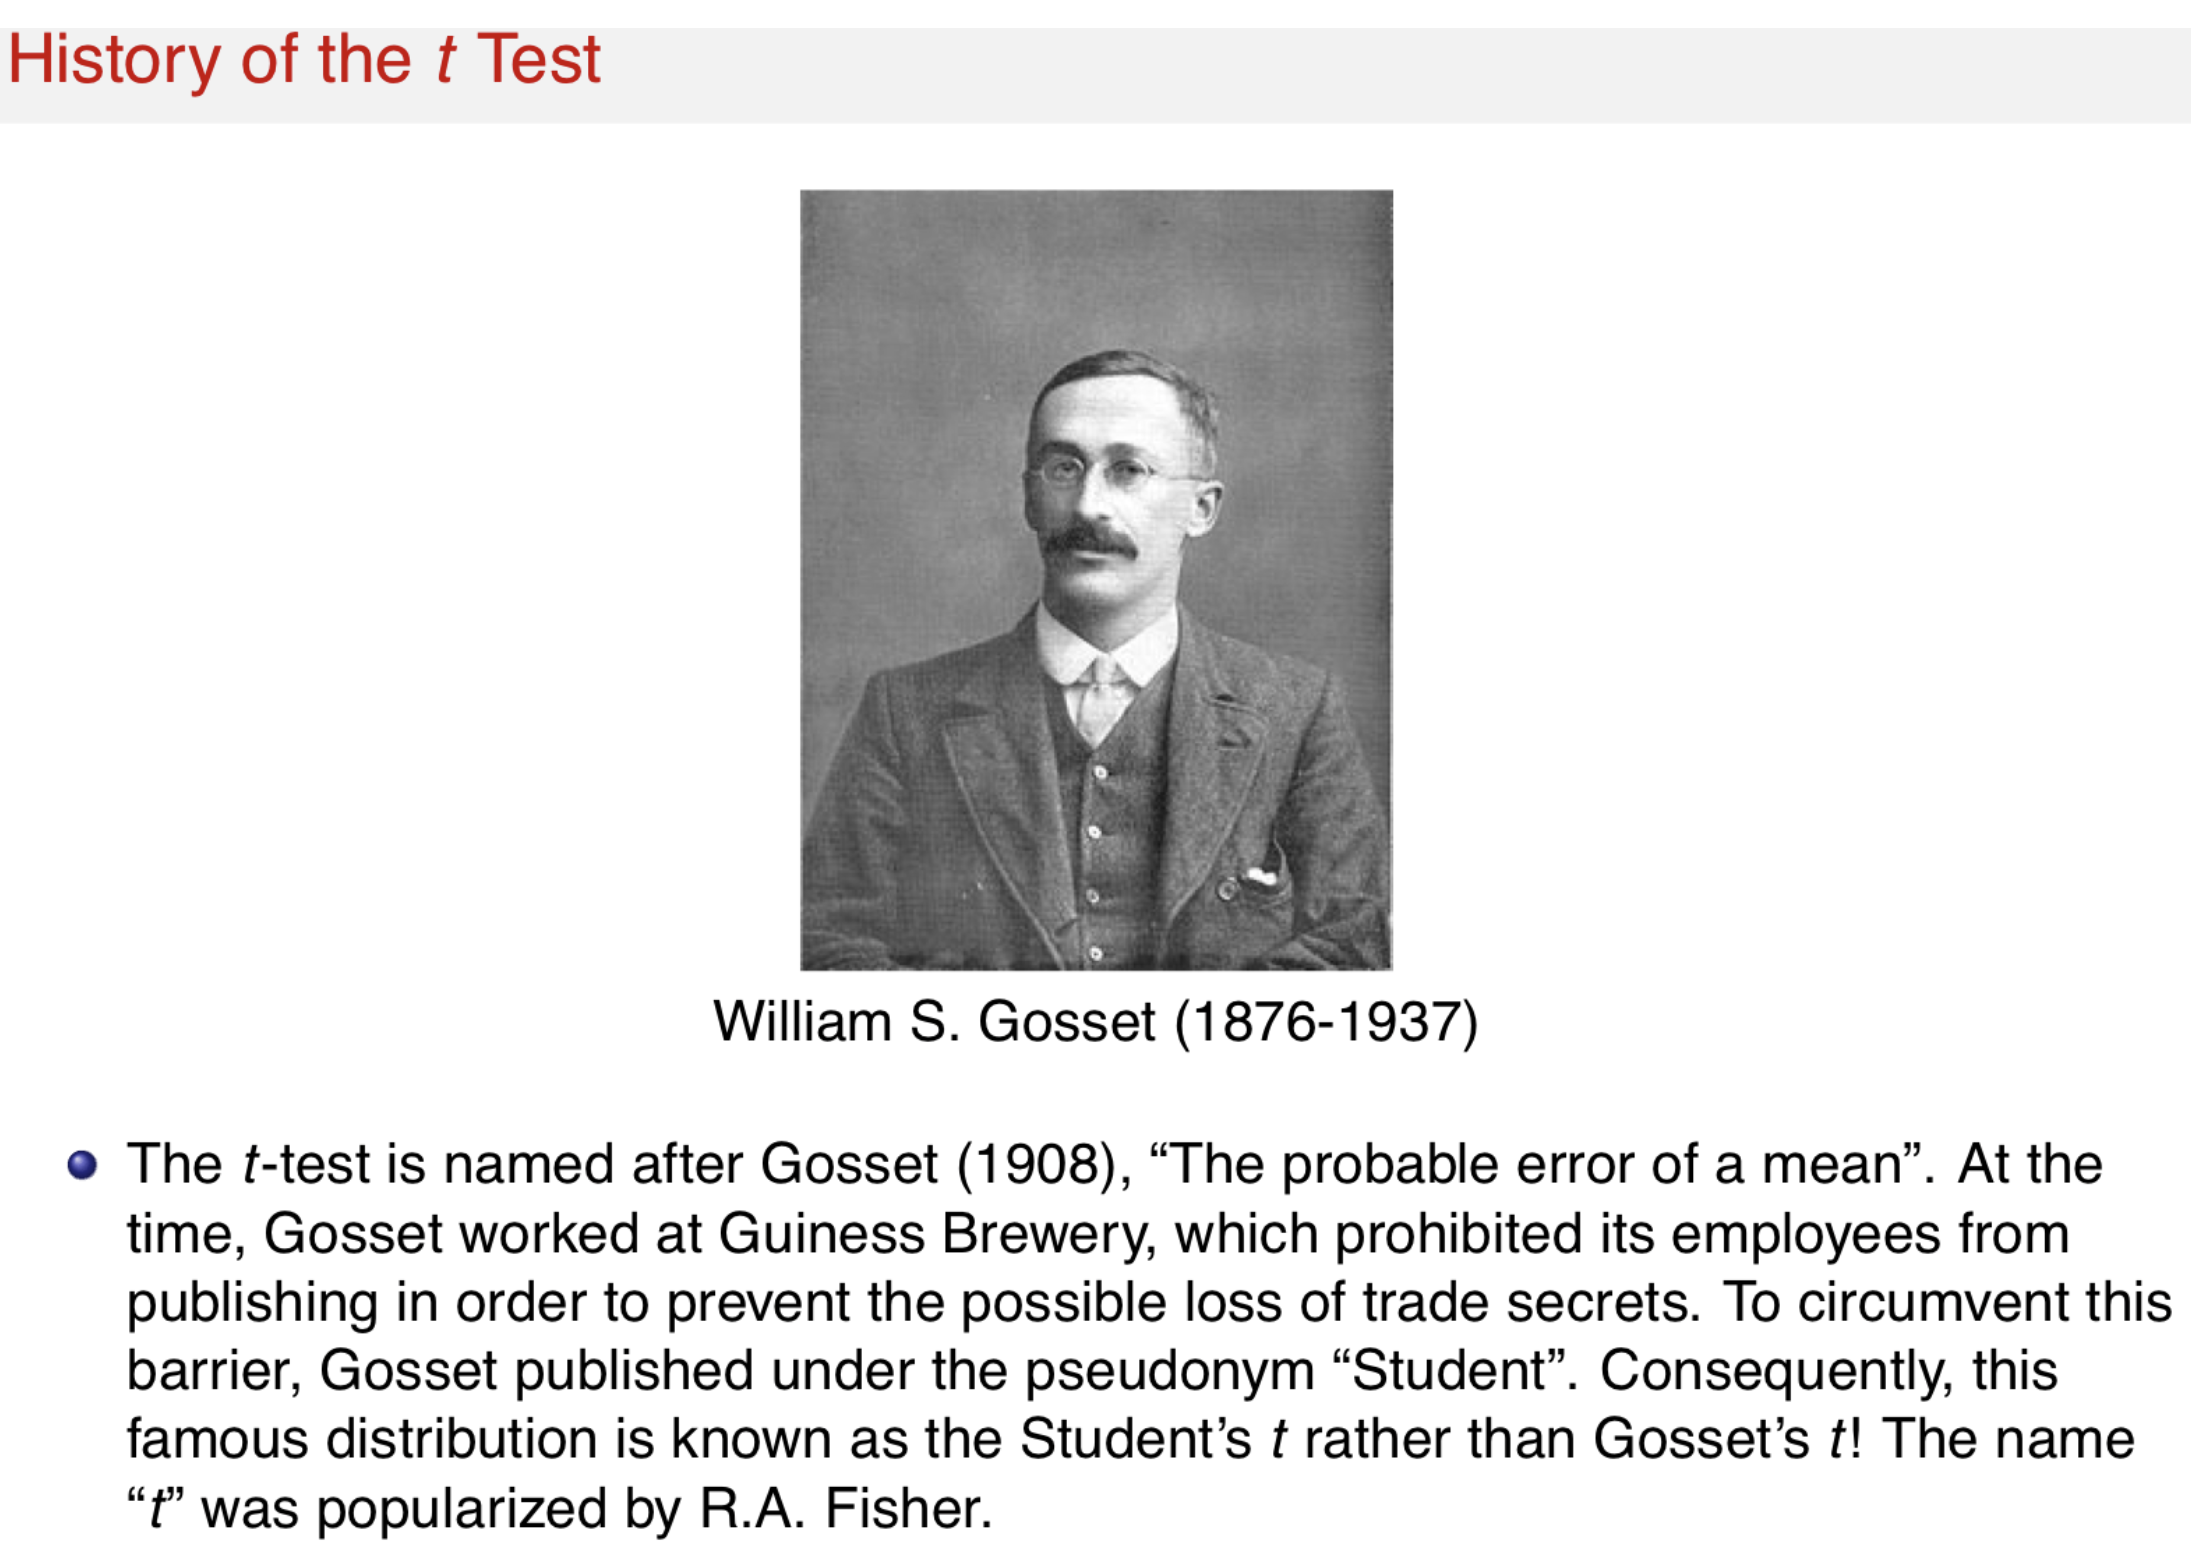
\includegraphics[width=1\textwidth]{fig6.png}
\end{figure}

\begin{figure}[H]
    \centering
    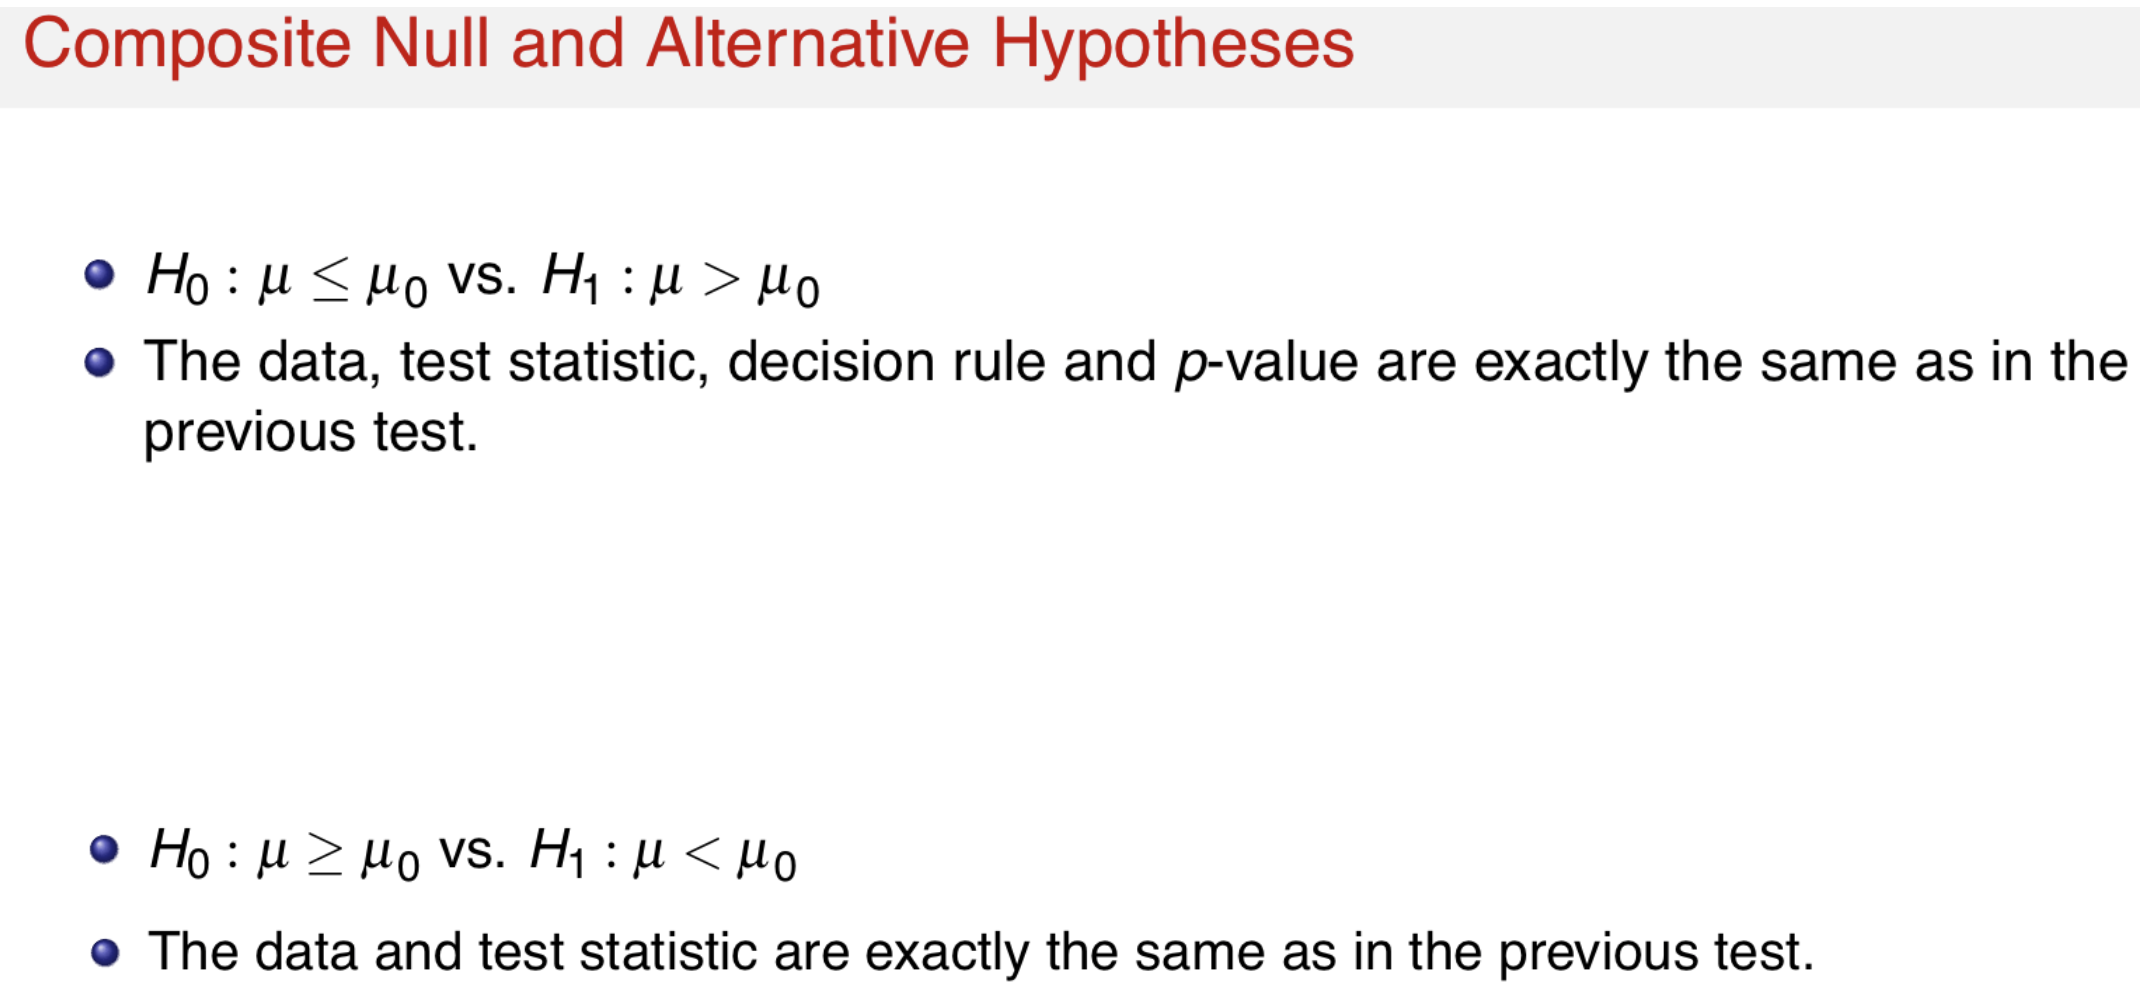
\includegraphics[width=1\textwidth]{fig7.png}
\end{figure}


\newpage
\section*{Schematic Summary}

\begin{figure}[H]
    \centering
    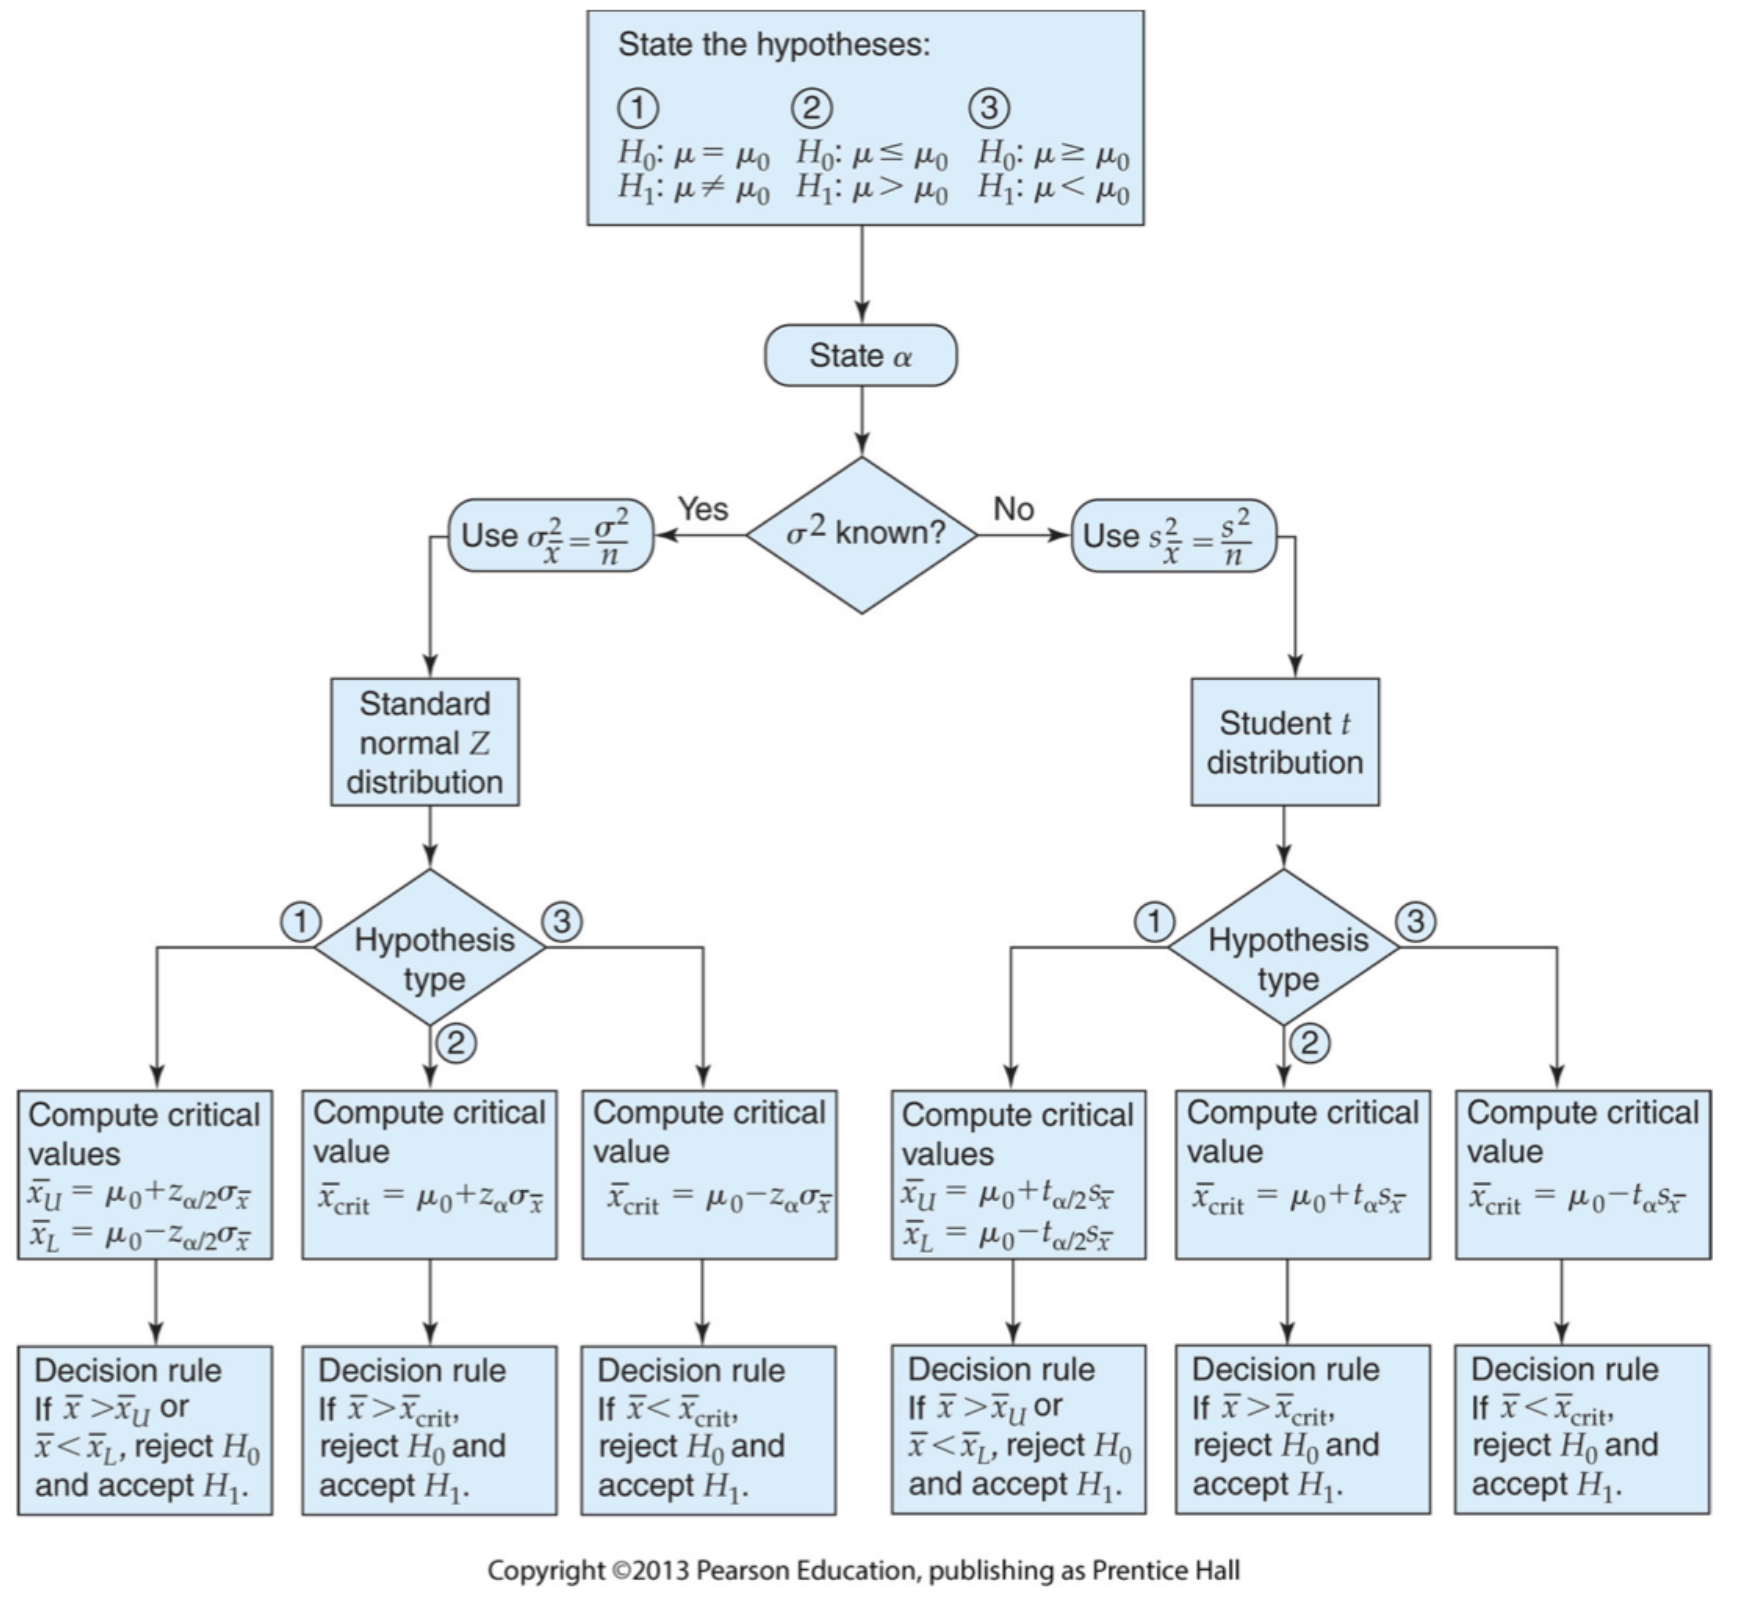
\includegraphics[width=1\textwidth]{fig8.png}
\end{figure}

\begin{figure}[H]
    \centering
    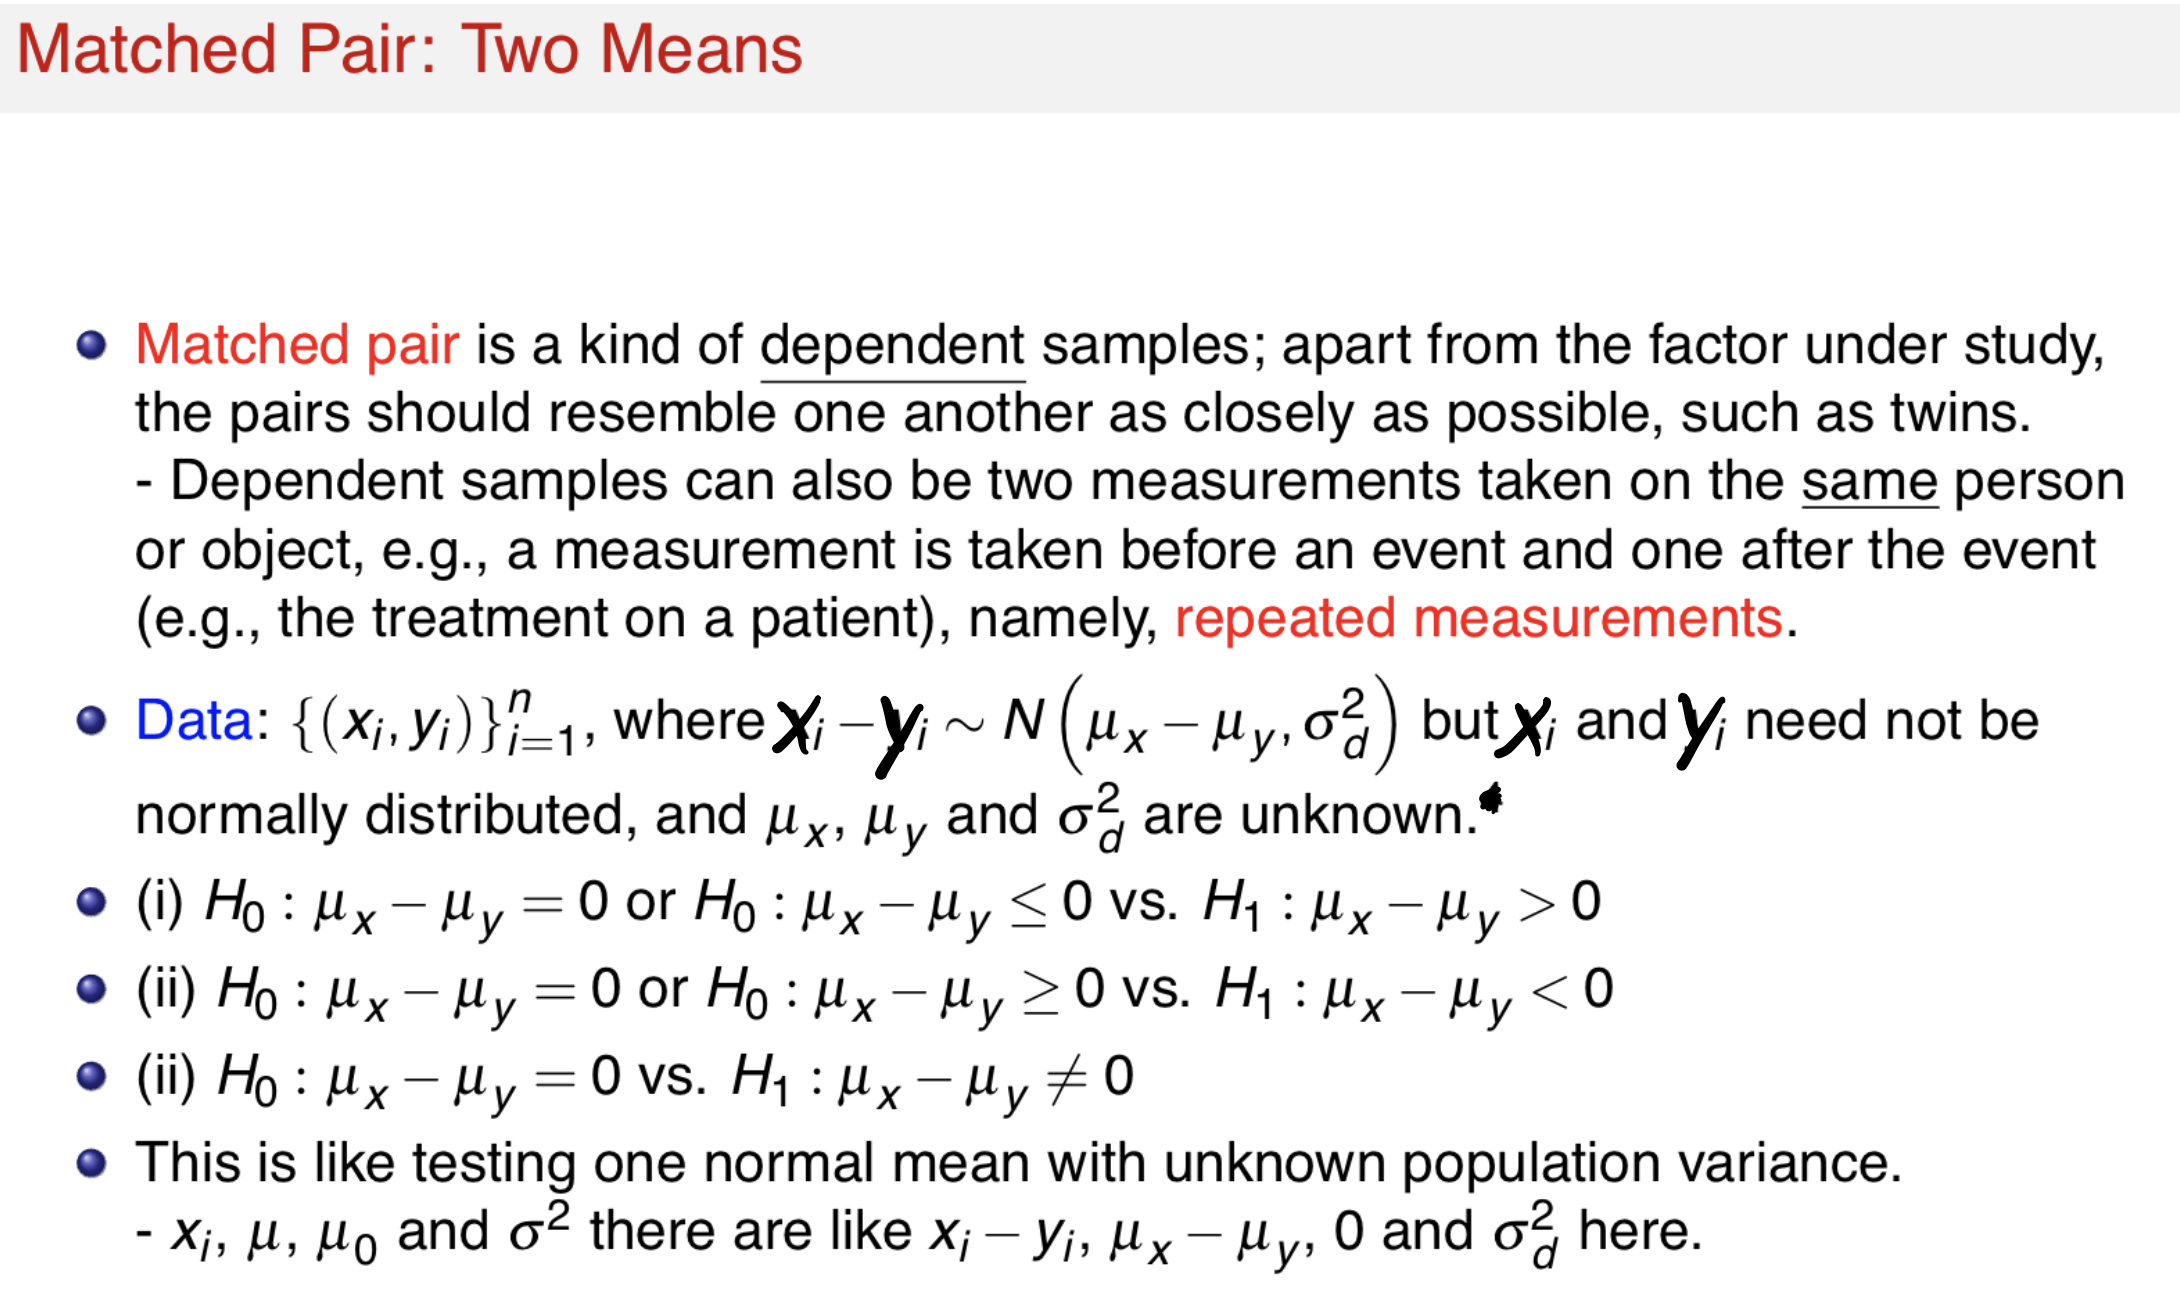
\includegraphics[width=1\textwidth]{fig9.png}
\end{figure}

\begin{figure}[H]
    \centering
    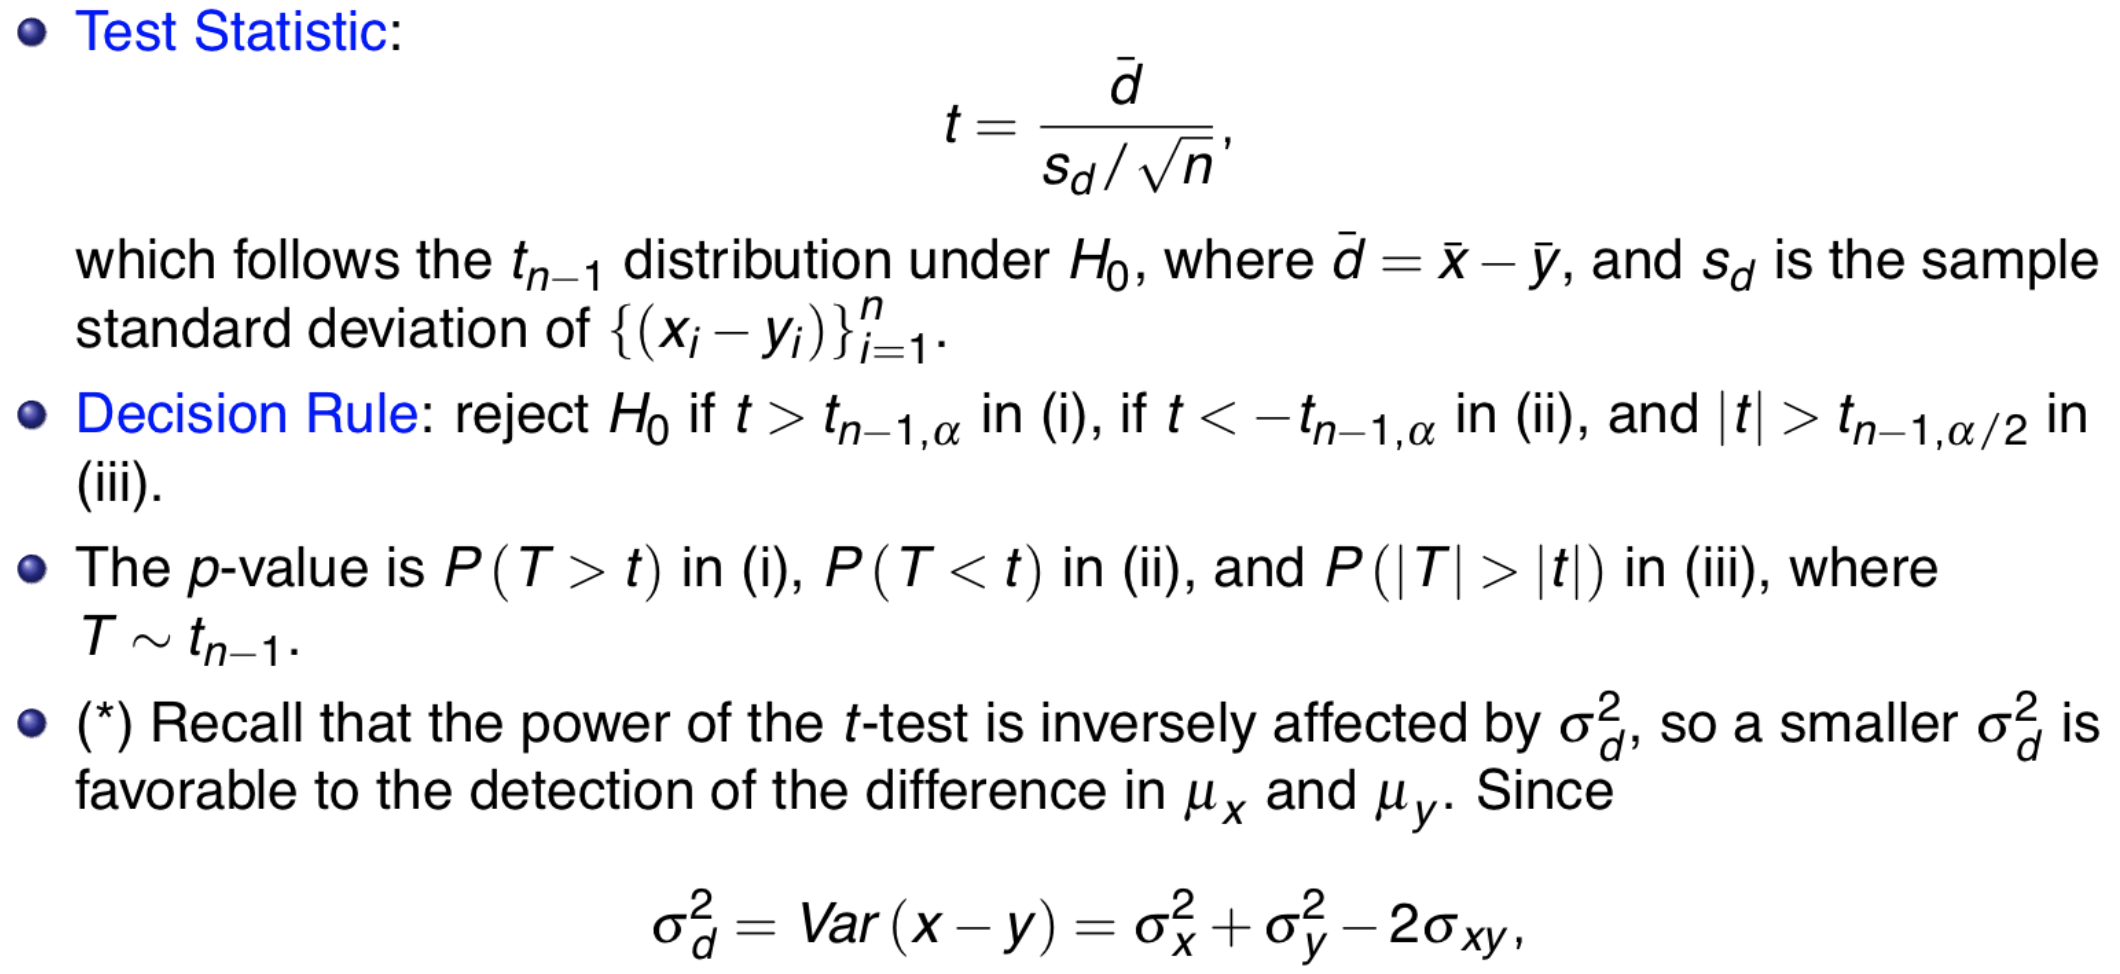
\includegraphics[width=1\textwidth]{fig10.png}
\end{figure}

\newpage

\section*{Example: Paired t-test}

\begin{itemize}
    \item Compare the effects of two soporific drugs.
    \item Each subject receives placebo, Drug 1, and Drug 2.
    \item Dependent variable: Number of hours of increased sleep.
    \item Drug 1 given to $n$ subjects, Drug 2 given to the same $n$ subjects.
    \item Study question: Is Drug 1 or Drug 2 more effective at increasing sleep?
    \begin{itemize}
        \item $H_0: \mu_d = 0$ \quad where $\mu_d = \mu_1 - \mu_2$
        \item $H_1: \mu_d \neq 0$
    \end{itemize}
\end{itemize}

\begin{center} % Center the table
\begin{tabular}{|c|c|c|c|} % Set text color to red for the last column
\hline
\textbf{Subject} & \textbf{Drug 1} & \textbf{Drug 2} & \textcolor{red}{\textbf{Diff (2-1)}} \\ 
\hline
1  & 0.7  & 1.9  & \textcolor{red}{1.2} \\
2  & -1.6 & 0.8  & \textcolor{red}{2.4} \\
3  & -0.2 & 1.1  & \textcolor{red}{1.3} \\
4  & -1.2 & 0.1  & \textcolor{red}{1.3} \\
5  & -0.1 & -0.1 & \textcolor{red}{0.0} \\
6  & 3.4  & 4.4  & \textcolor{red}{1.0} \\
7  & 3.7  & 5.5  & \textcolor{red}{1.8} \\
8  & 0.8  & 1.6  & \textcolor{red}{0.8} \\
9  & 0.0  & 4.6  & \textcolor{red}{4.6} \\
10 & 2.0  & 3.4  & \textcolor{red}{1.4} \\
\hline
\textbf{Mean} & 0.75 & 2.33 & \textcolor{red}{1.58} \\
\textbf{SD}   & 1.79 & 2.0  & \textcolor{red}{1.2} \\
\hline
\end{tabular}
\end{center}

\begin{figure}[H]
    \centering
    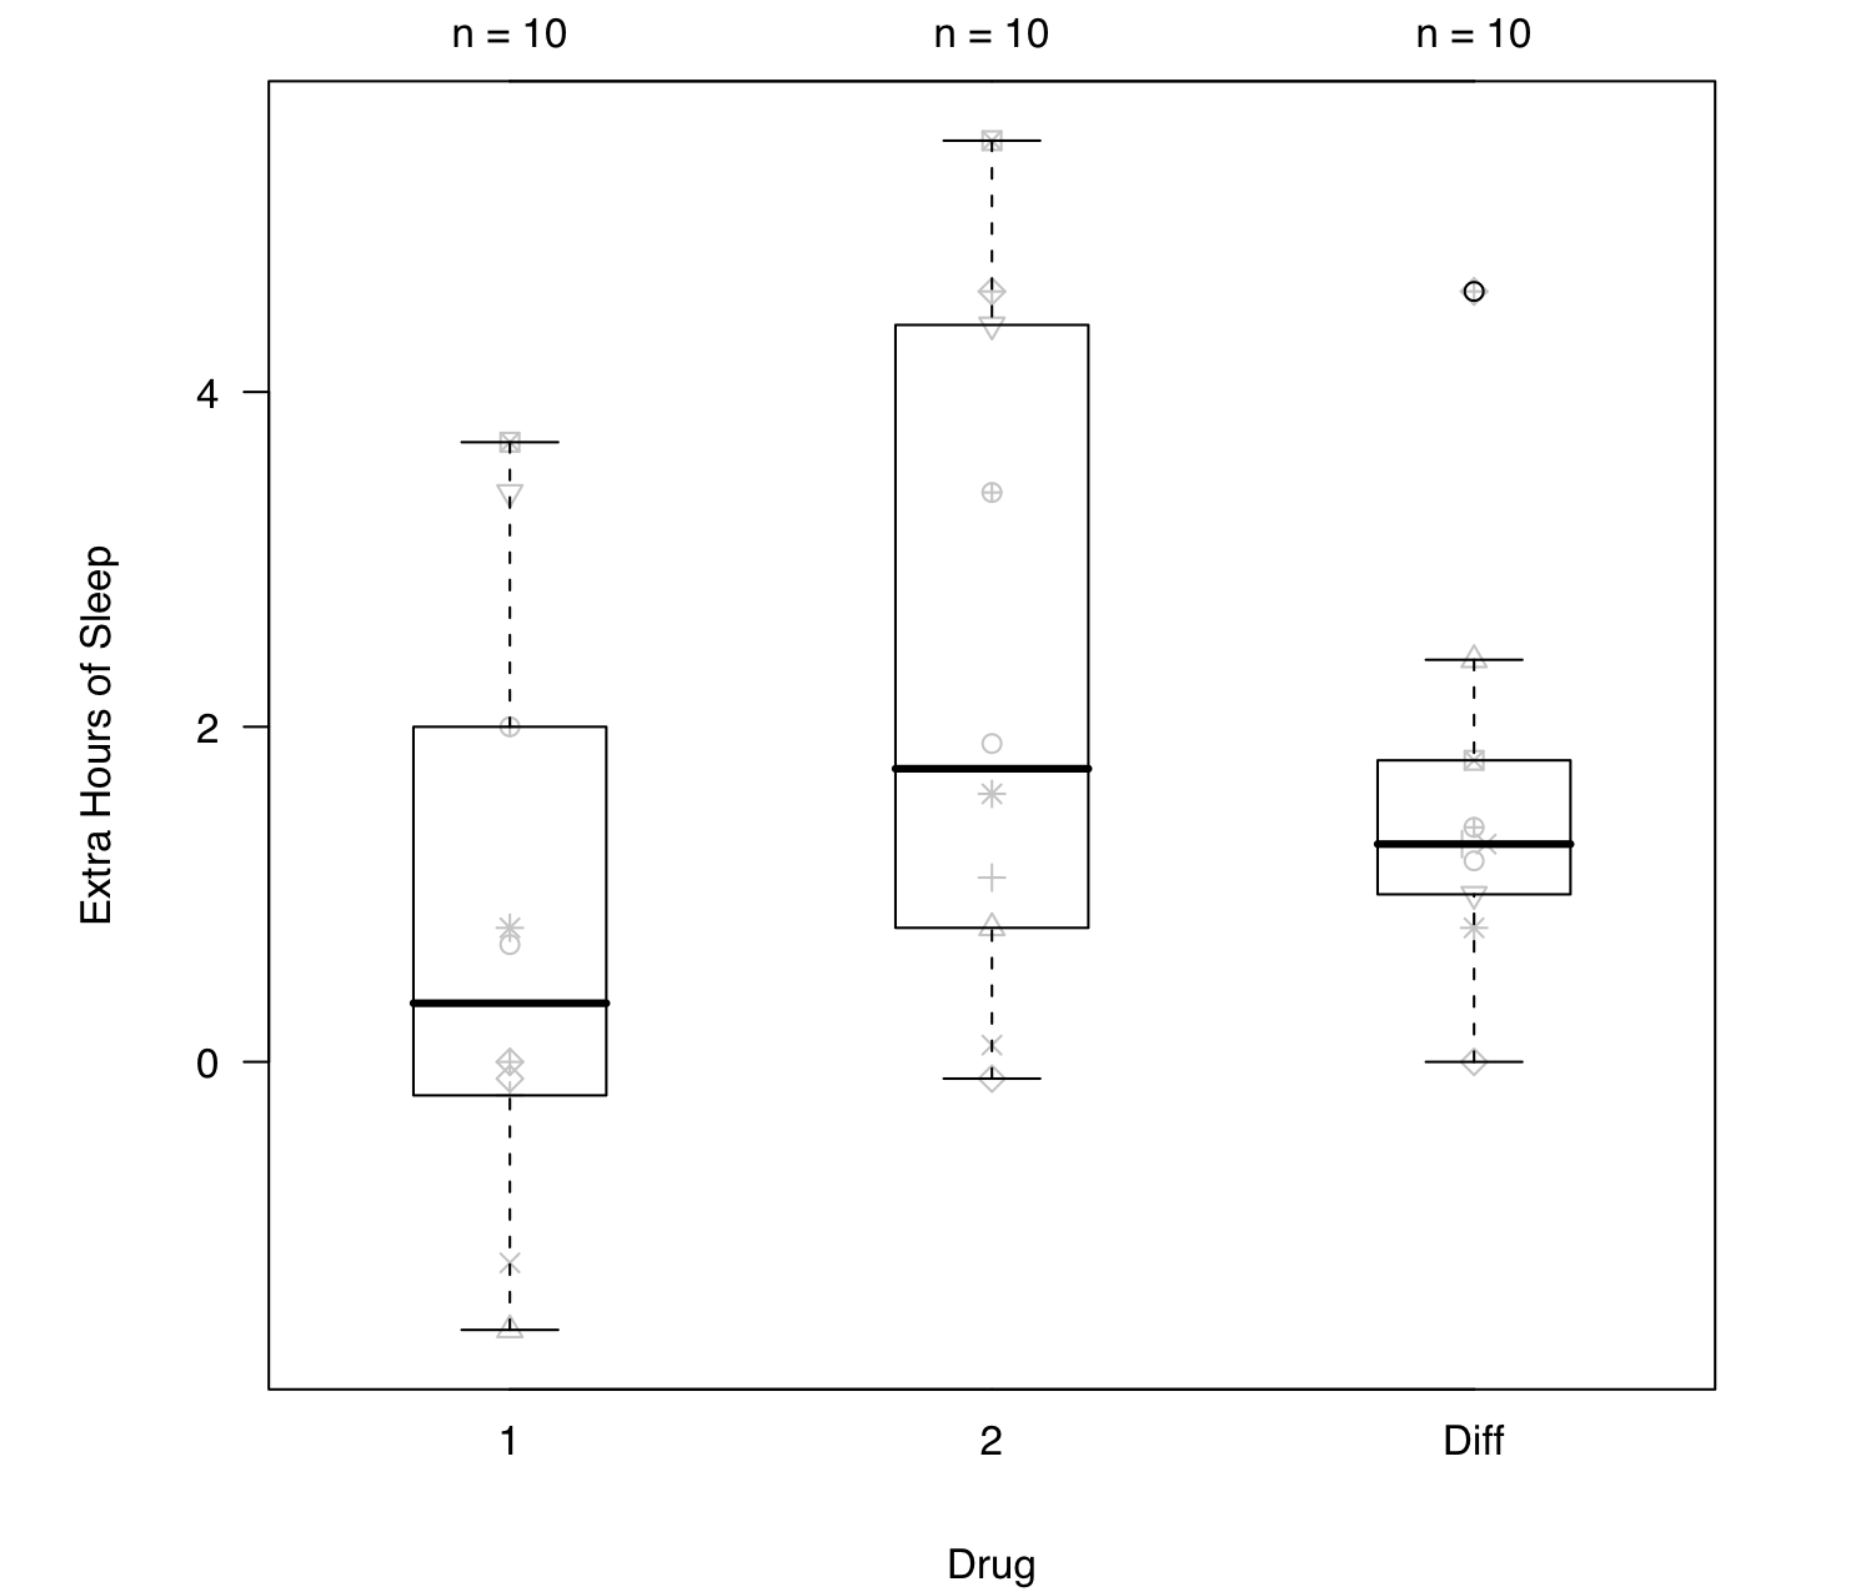
\includegraphics[width=0.8\textwidth]{fig11.png}
\end{figure}

\begin{figure}[H]
    \centering
    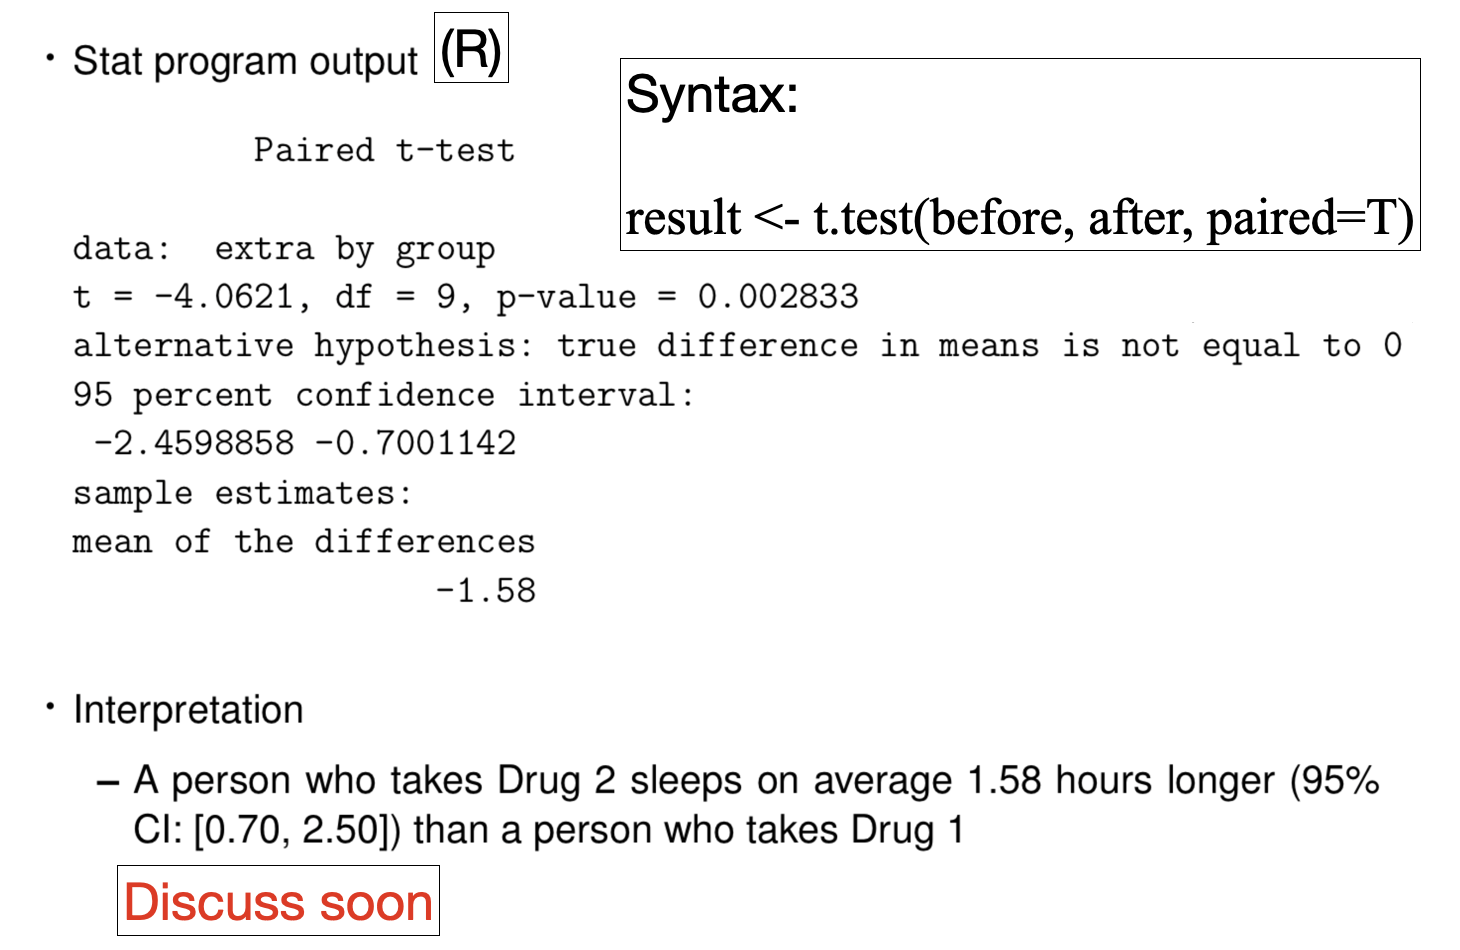
\includegraphics[width=1\textwidth]{fig12.png}
\end{figure}

\section*{Two Sample t-test}
\textbf{Sampling model:}
\[
Y_{1A}, \ldots, Y_{n_AA} \sim \text{i.i.d. } \mathcal{N}(\mu_A, \sigma^2)
\]
\[
Y_{1B}, \ldots, Y_{n_BB} \sim \text{i.i.d. } \mathcal{N}(\mu_B, \sigma^2)
\]
\[\textcolor{red}{\text{note that:} \sigma^2 \text{equal variances assumed}}\]
\[
H_0: \mu_A = \mu_B
\]
\[
H_1: \mu_A \neq \mu_B
\]

\textbf{Recall:}
\[
\overline{Y}_B - \overline{Y}_A \sim N(\mu_B - \mu_A, \sigma^2 \left( \frac{1}{n_A} + \frac{1}{n_B} \right))
\]

If $H_0$ is true:
\[
\overline{Y}_B - \overline{Y}_A \sim N(0, \sigma^2 \left( \frac{1}{n_A} + \frac{1}{n_B} \right))
\]

\[\textcolor{red}{\text{How to get plug-in estimates for }\sigma^2 ?}\]

\textbf{Consider: }

\textcolor{red}{$s_p^2$: pooled variance}
\[
s_p^2 = \frac{\sum_{i=1}^{n_A} (Y_i - \bar{Y}_A)^2 + \sum_{i=1}^{n_B} (Y_i - \bar{Y}_B)^2}{(n_A-1) + (n_B-1)}
\]
\[
= \frac{(n_A-1)s_A^2 + (n_B-1)s_B^2}{(n_A-1) + (n_B-1)}
\]

\newpage

\textbf{This generates two-sample t-statistic}
\[\textcolor{red}{0 \text{ refers to } H_0 : \mu_A = \mu_B}\]
\[
t(Y_A, Y_B) = \frac{(\overline{Y}_B - \overline{Y}_A) - 0}{s_p \sqrt{\frac{1}{n_A} + \frac{1}{n_B}}}
\]
\[
\overset{H_0}{\sim}  t_{n_A + n_B - 2}
\]

\section*{Numerical Example (2 trt data again) } 
\begin{figure}[H]
    \centering
    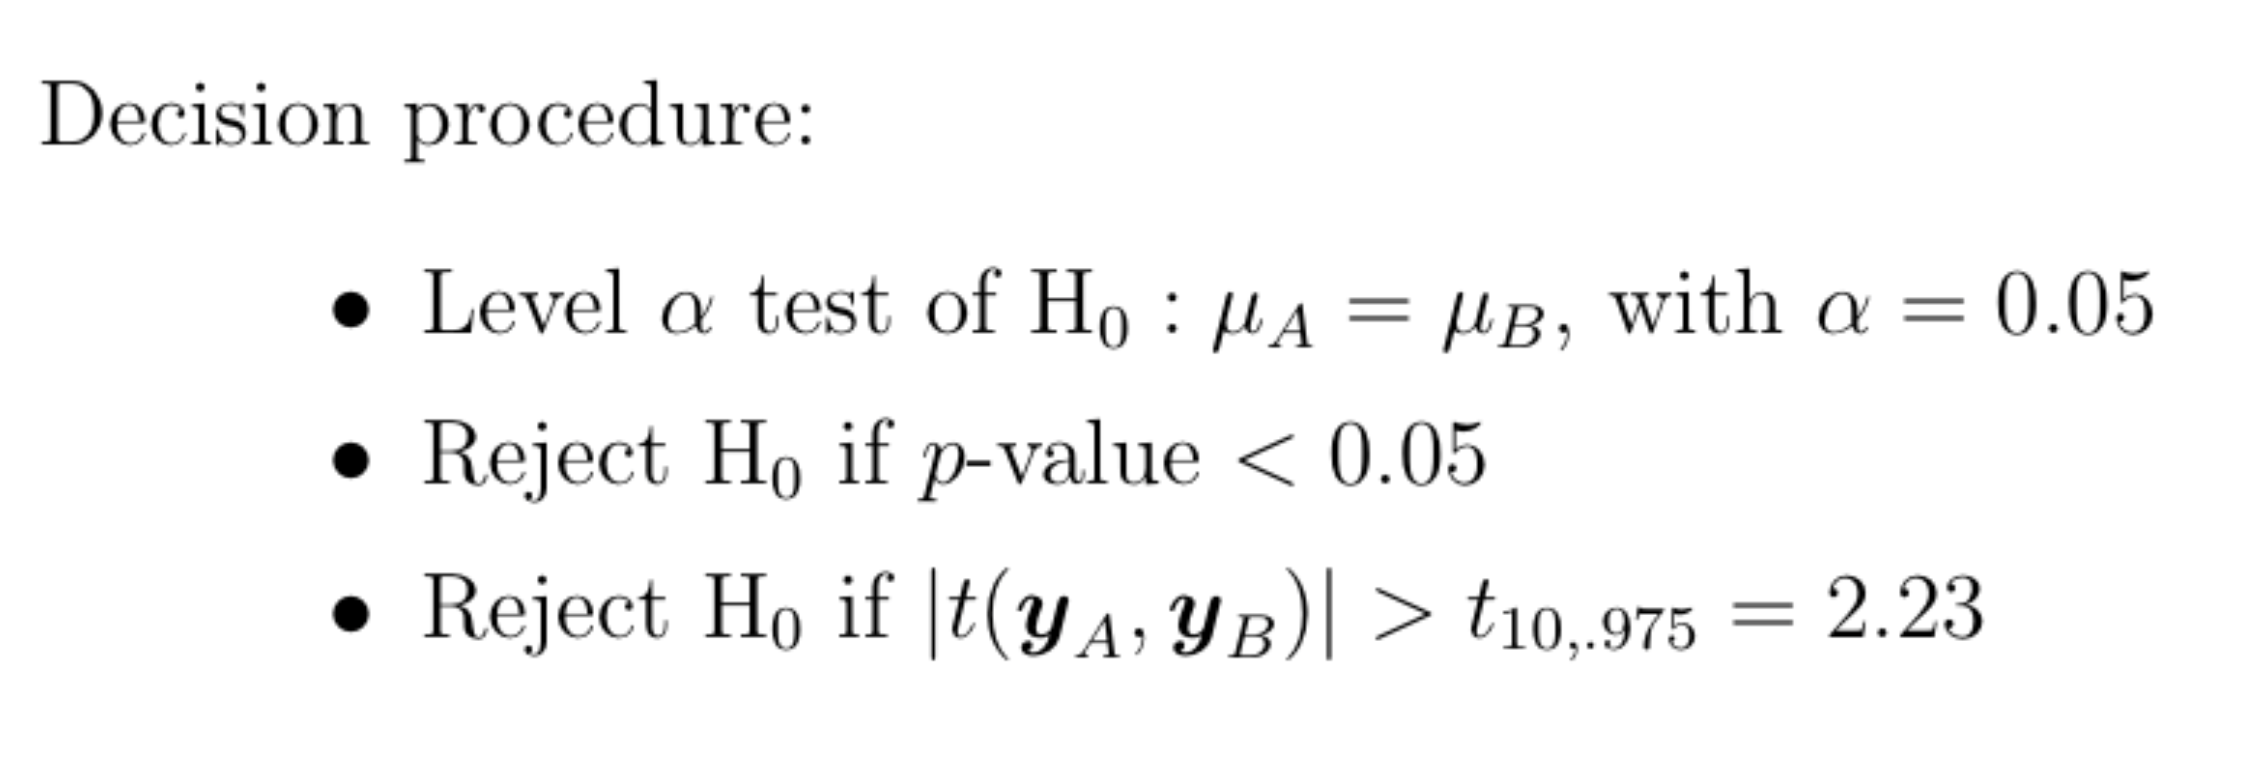
\includegraphics[width=1\textwidth]{fig13.png}
\end{figure}

\begin{figure}[H]
    \centering
    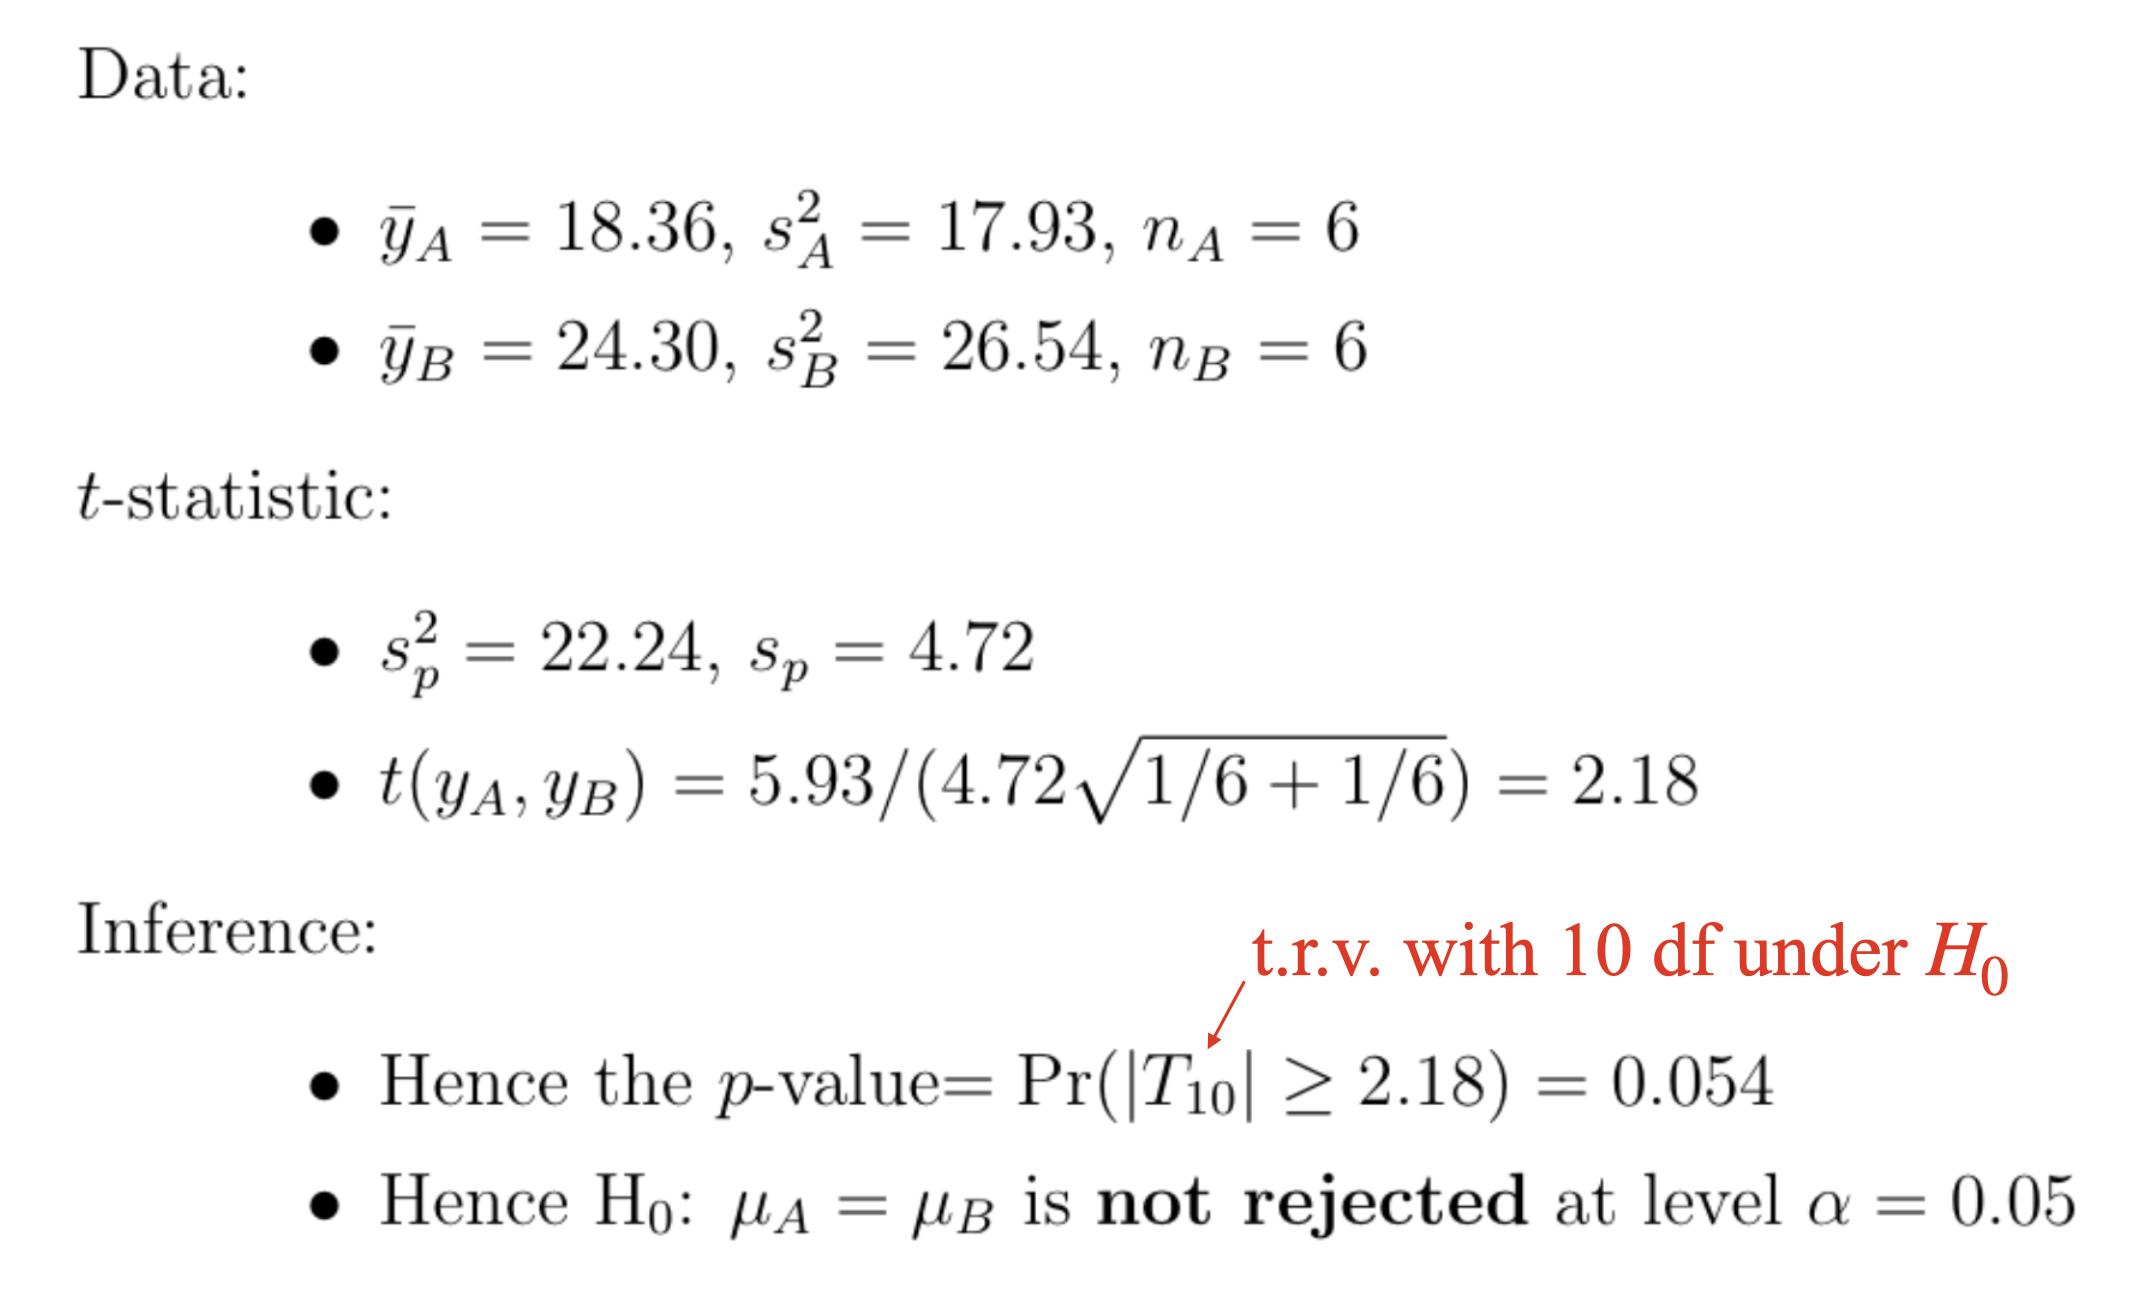
\includegraphics[width=1\textwidth]{fig14.png}
\end{figure}

\begin{figure}[H]
    \centering
    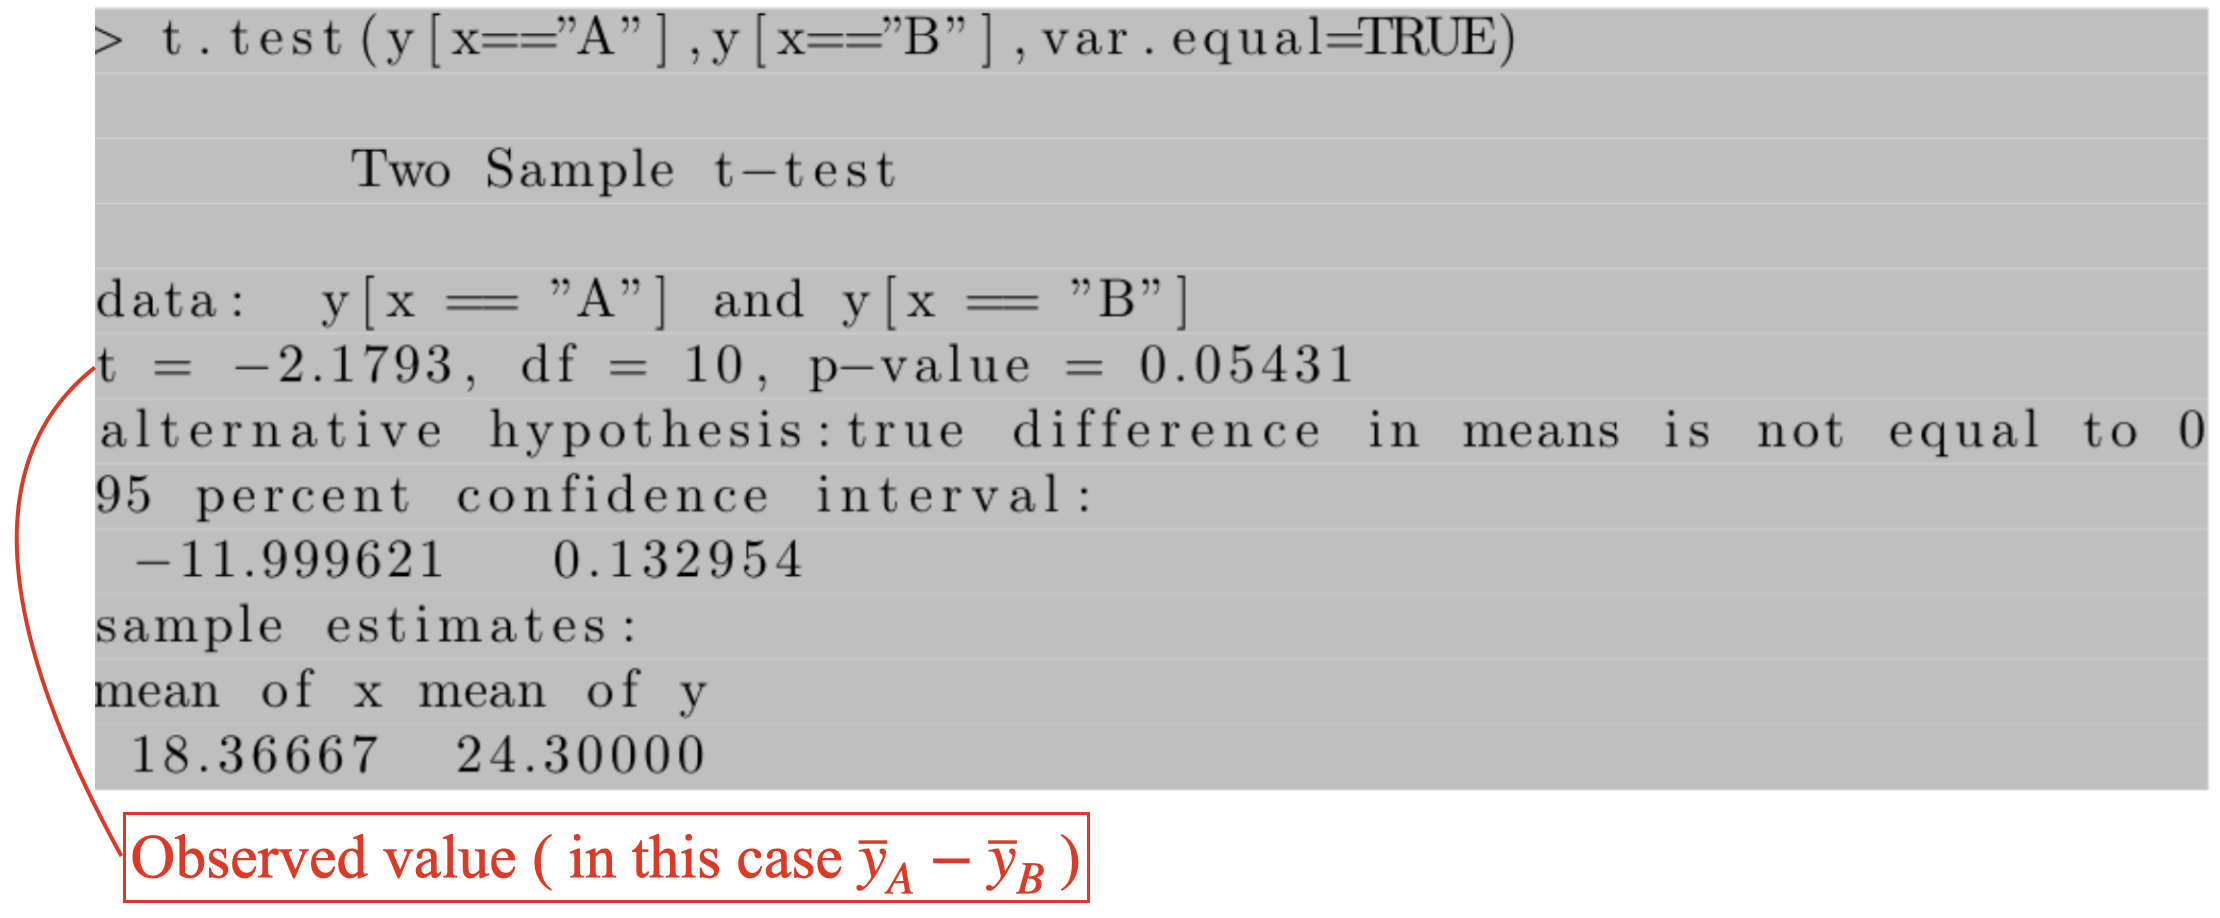
\includegraphics[width=1\textwidth]{fig15.png}
\end{figure}

\begin{figure}[H]
    \centering
    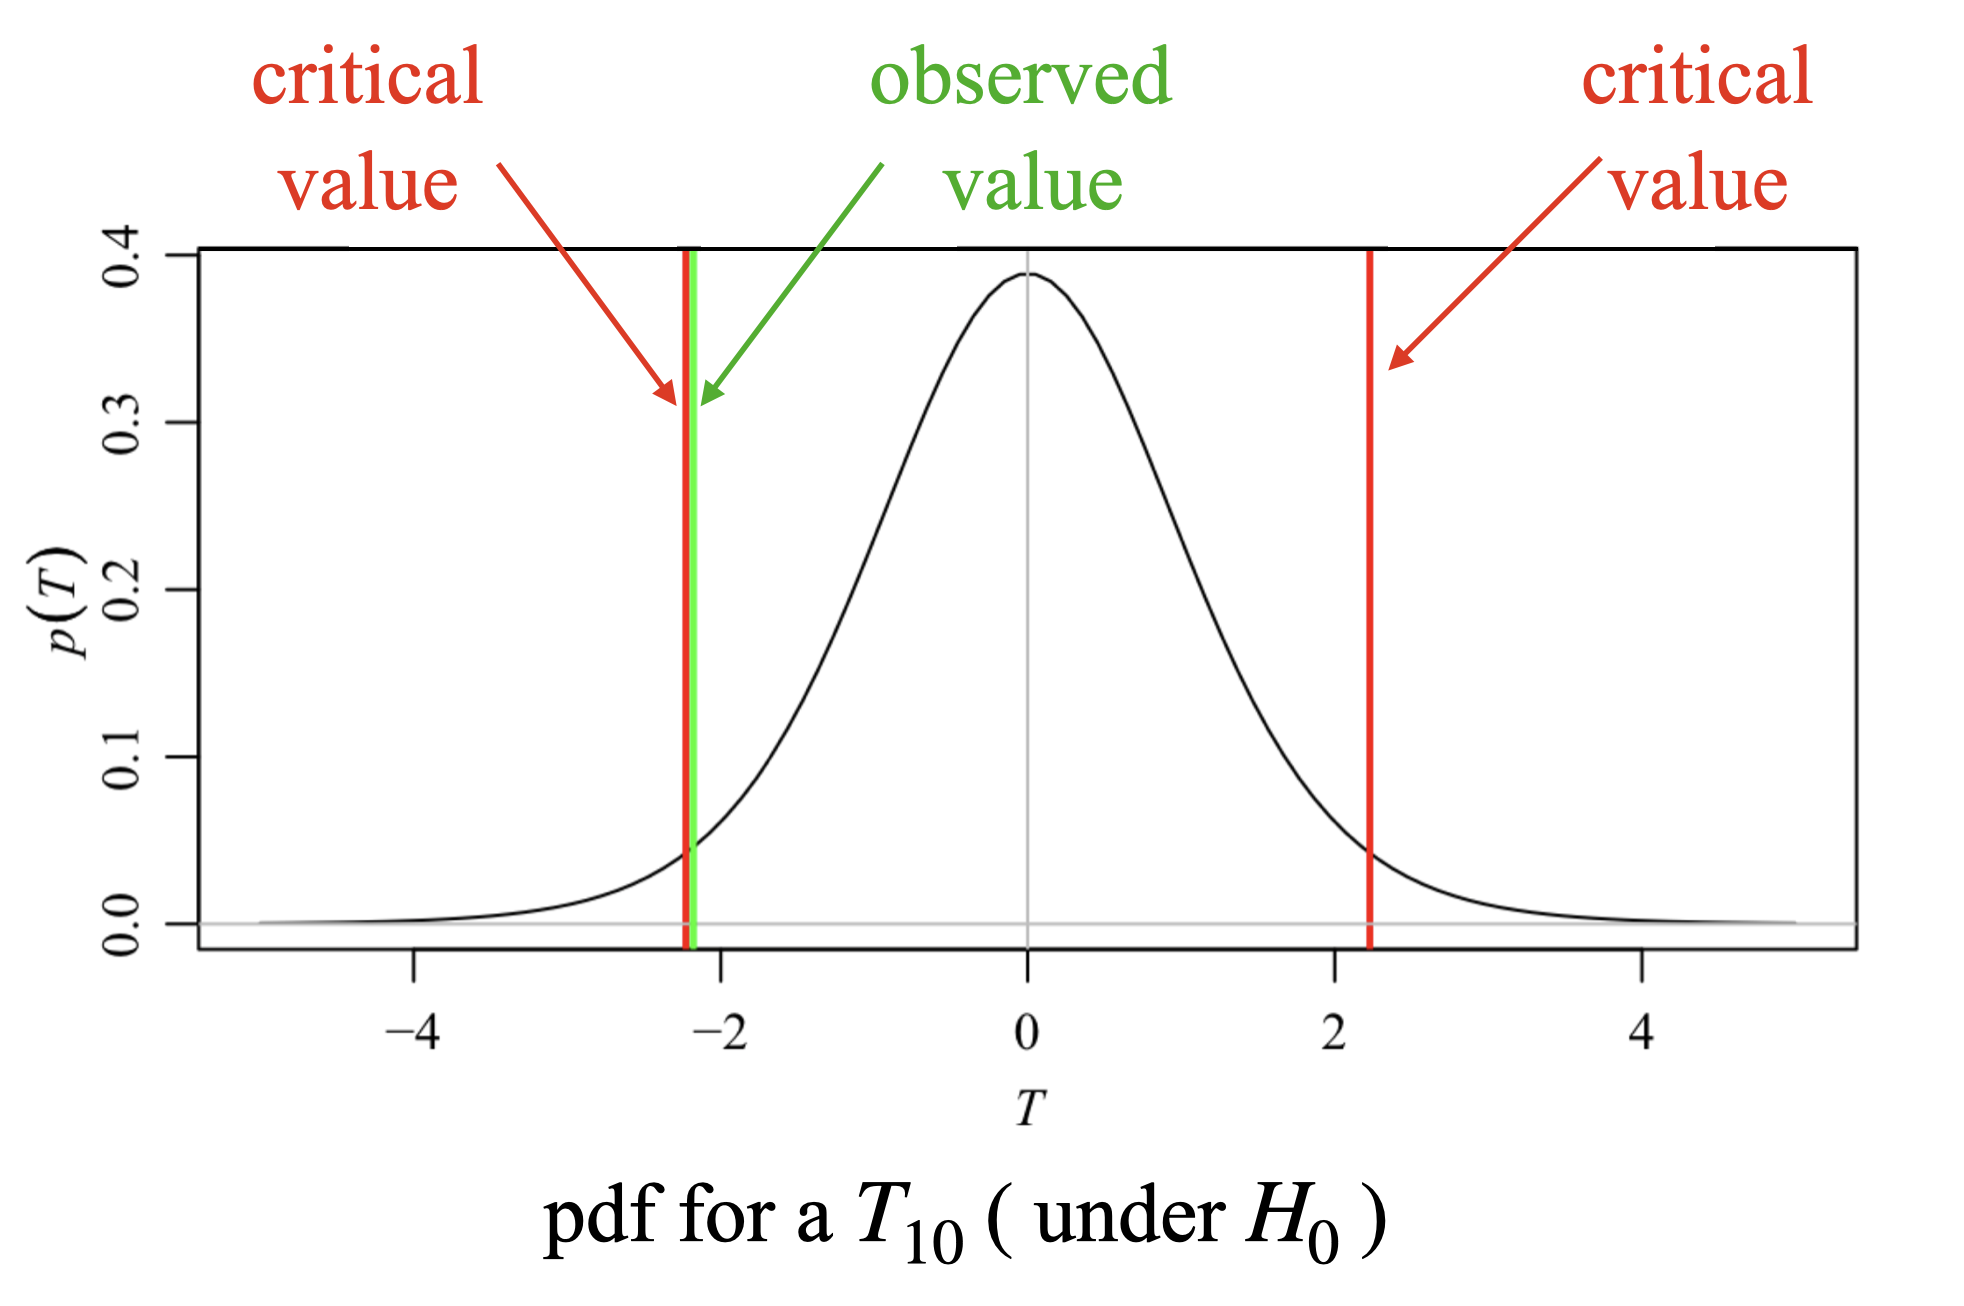
\includegraphics[width=1\textwidth]{fig16.png}
\end{figure}

\newpage

\section*{Comparison to Randomization Test} 

\begin{figure}[H]
    \centering
    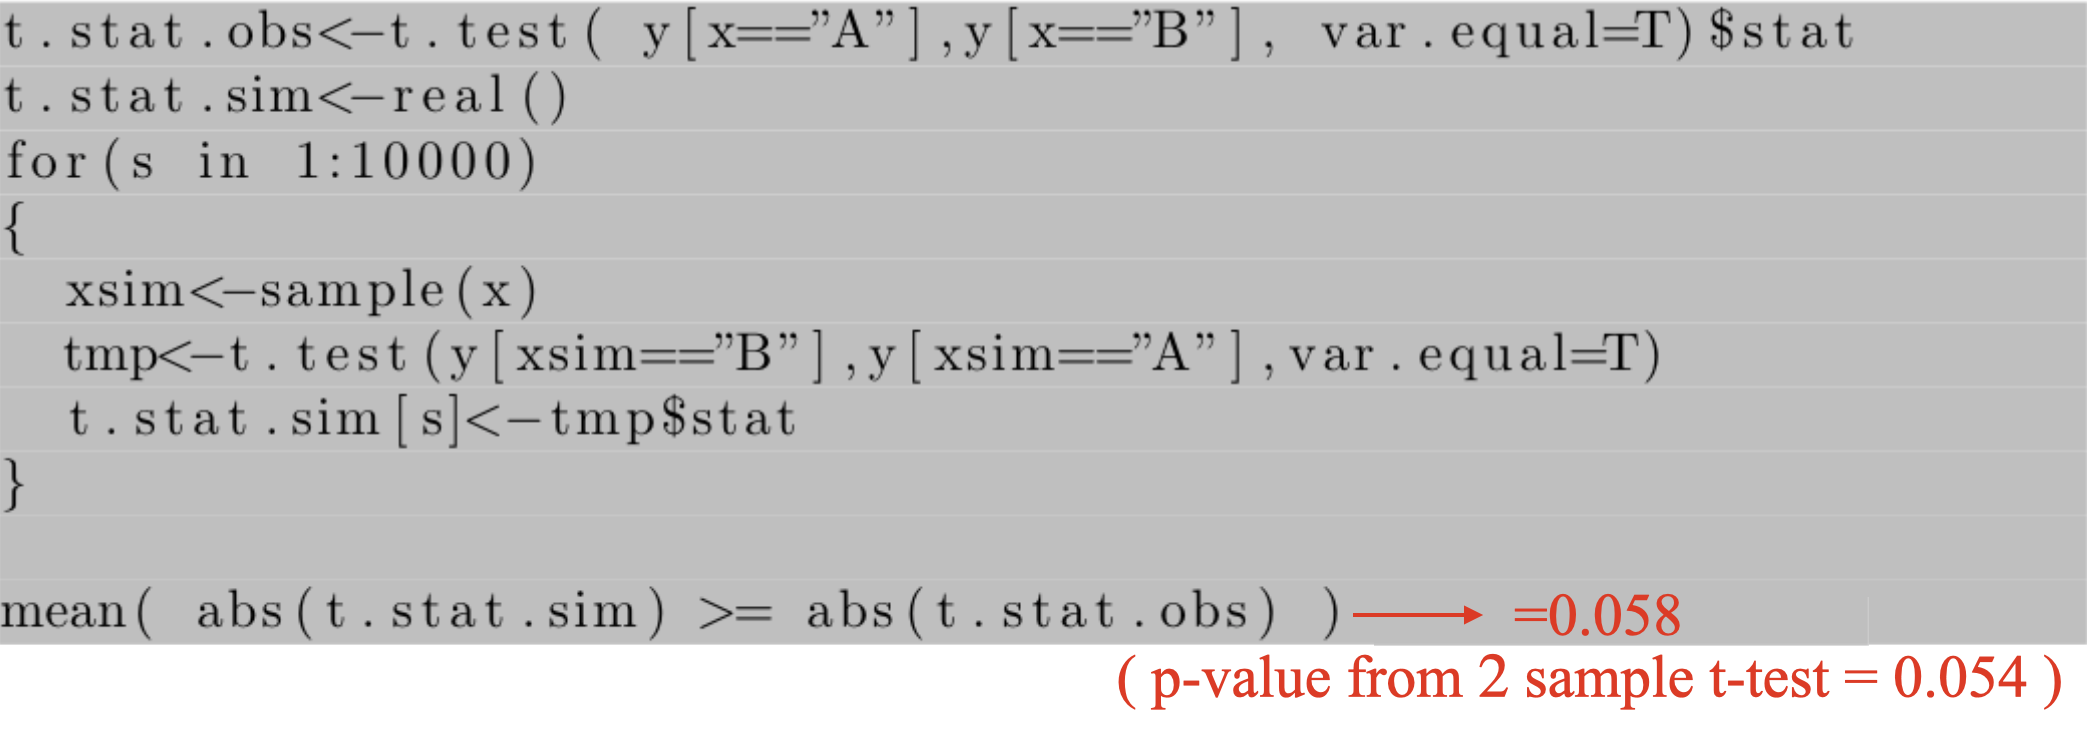
\includegraphics[width=1\textwidth]{fig17.png}
\end{figure}

\begin{figure}[H]
    \centering
    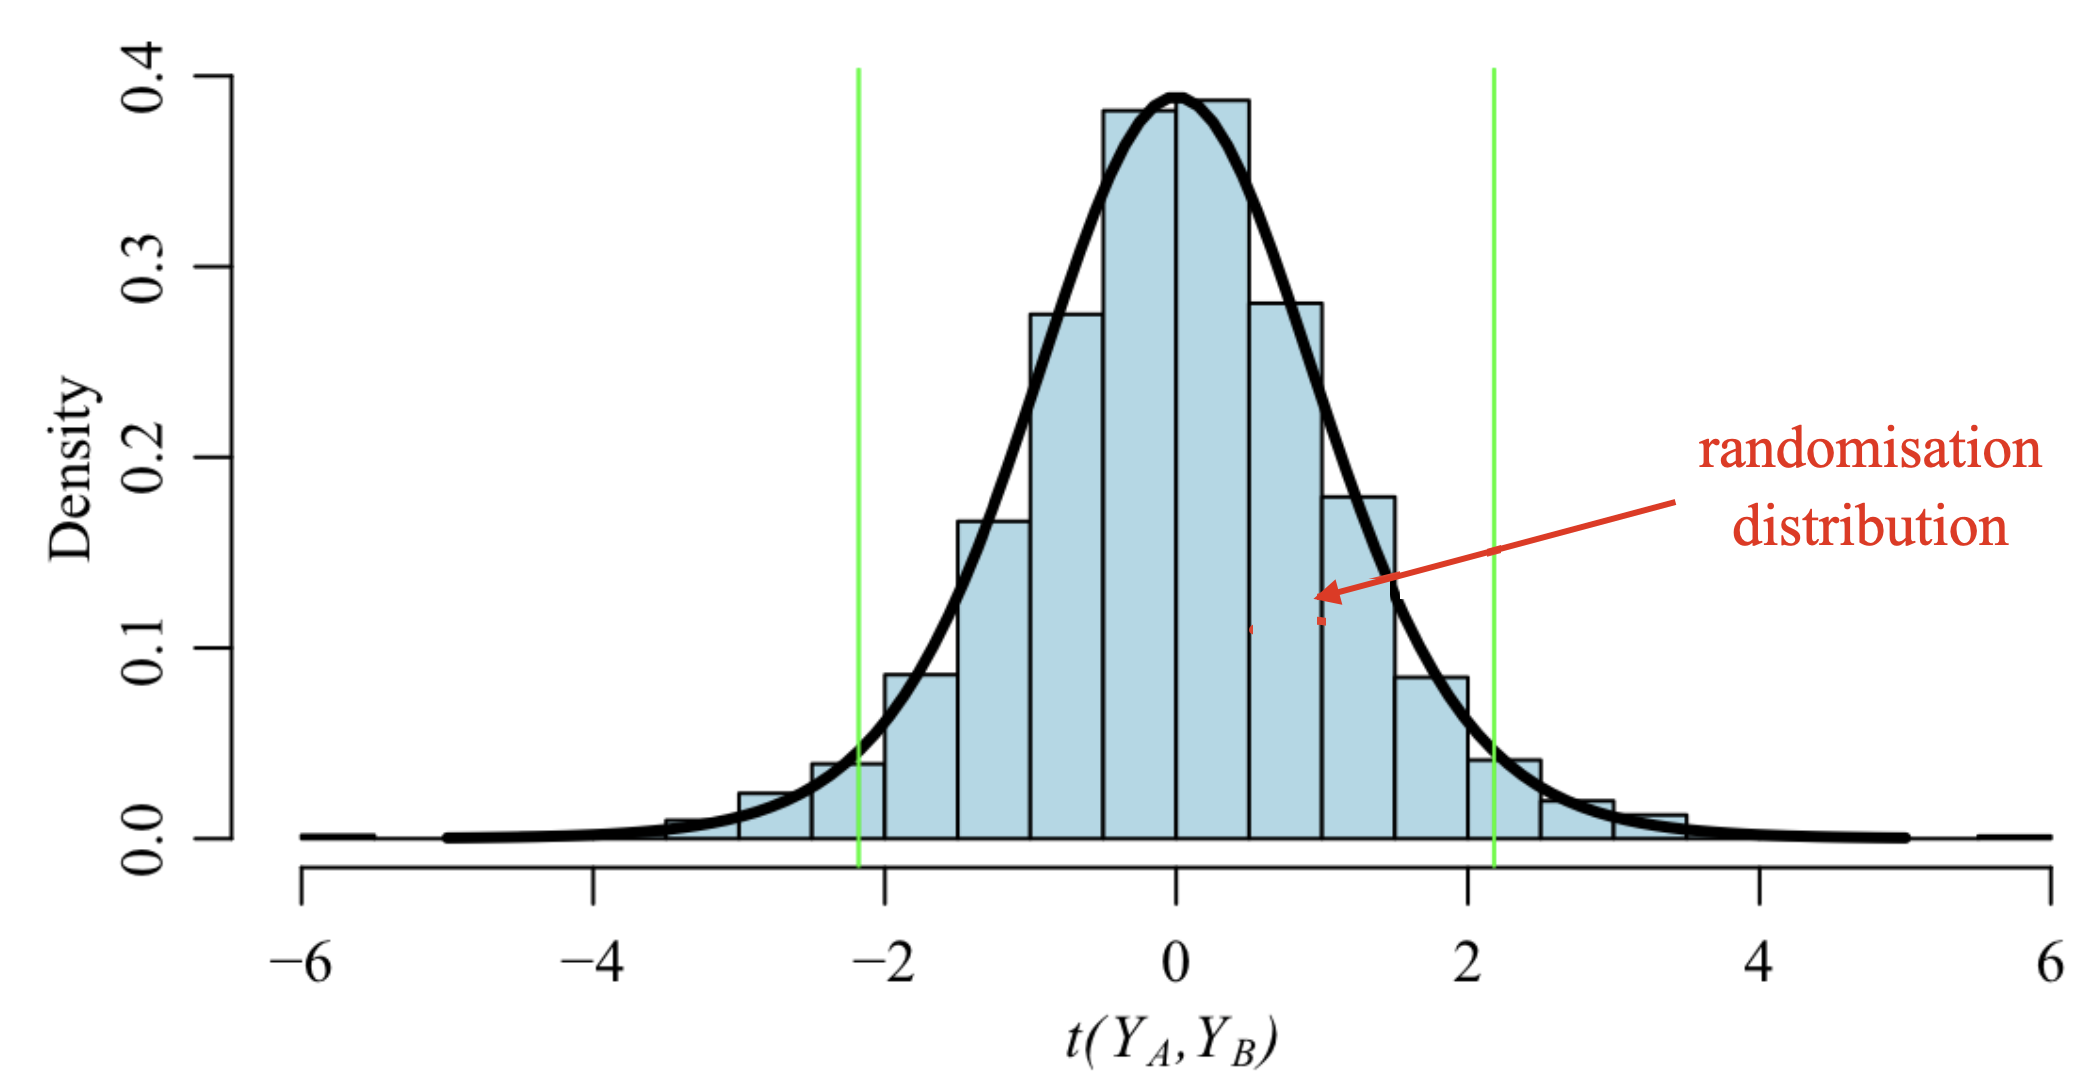
\includegraphics[width=1\textwidth]{fig18.png}
\end{figure}

\newpage

\textbf{Is there concordance between the two approaches surprising?}

\textbf{Assumptions: }Under $H_0$

\begin{itemize}
    \item \textbf{Randomization Test:}
    \begin{enumerate}
        \item Treatments are randomly assigned
    \end{enumerate}
    
    \item \textbf{t-test:}
    \begin{enumerate}
        \item Data are independent samples
        \item Each population is normally distributed
        \item The two populations have the same variance
    \end{enumerate}
\end{itemize}

\textbf{Imagined Universes:}

\begin{itemize}
    \item Randomization Test: \textbf{Numerical responses} remain \textbf{fixed}, we imagine only alternative treatment assignments.

    \item t-test: \textbf{Treatment assignments} remain \textbf{fixed}, we imagine an alternative sample of experimental units and/or conditions, giving \textbf{different numerical responses}.
\end{itemize}

\textbf{Inferential Context / Type of Generalization}

\begin{itemize}
    \item Randomization Test: Inference is specific to our particular experimental units and conditions.
    \item t-test: Under our assumptions, inference claims to be \textbf{generalizable }to other units / conditions, i.e., to a larger population.
\end{itemize}

Yet the numerical results are often nearly identical.

\newpage

\textbf{Keep the following concepts clear:}

\begin{itemize}
    \item \textbf{t-statistic}: a scaled difference in sample means, computed from the data.
    
    \item \textbf{t-distribution}: the probability distribution of a normal random variable divided by the square-root of a $\chi^2$ random variable.
    
    \item \textbf{t-test}: a comparison of a t-statistic to a t-distribution.
    
    \item \textbf{randomization distribution}: the probability distribution of a test statistic under random treatment reassignments and $H_0$.
    
    \item \textbf{randomization test}: a comparison of a test statistic to its randomization distribution.
    
    \item \textbf{randomization test with the t-statistic}: a comparison of the t-statistic to its randomization distribution.
\end{itemize}

\section*{Checking Assumptions}
Two sample t-test assumes:
\begin{itemize}
    \item[a)] $\mu_A = \mu_B$ (to derive sampling distribution under $H_0$)
    \item[b)] $\sigma^2_A = \sigma^2_B$
    \item[c)] $p_A$ and $p_B$ are normal distributions
\end{itemize}
Thus rejecting $H_0 \Rightarrow a)$ is not true,

$\therefore$ want to check $b)$ and $c)$.

\section*{Checking Normality}
- Use normal probability plot.\\
- Idea: order observed observations within each group.
\[
Y_{(1)A}, \cdots , Y_{(n_A)A}; \quad Y_{(1)B}, \cdots , Y_{(n_B)B}
\]

\noindent Compare these \textcolor{blue}{sample quantiles} to theoretical quantiles of a normal distribution ($N(0, 1)$ for convenience).
\[
Z_{\left( \frac{1}{n_A} - \frac{1}{2} \right)} \leq Z_{\left( \frac{2}{n_A} - \frac{1}{2} \right)} \leq \dots \leq Z_{\left( \frac{k}{n_A} - \frac{1}{2} \right)}
\]
\[\text{where} \quad P\left(Z \leq Z_{\left(\frac{k}{n_A} - \frac{1}{2}\right)}\right) = \frac{k}{n_A} - \frac{1}{2}
\]

\textcolor{blue}{[and similarly for the \(Y_{iB}\) observations ]} \\

Then plot one against the other. 

If normality holds, the relationship should be approximately linear.\\

\begin{figure}[H]
    \centering
    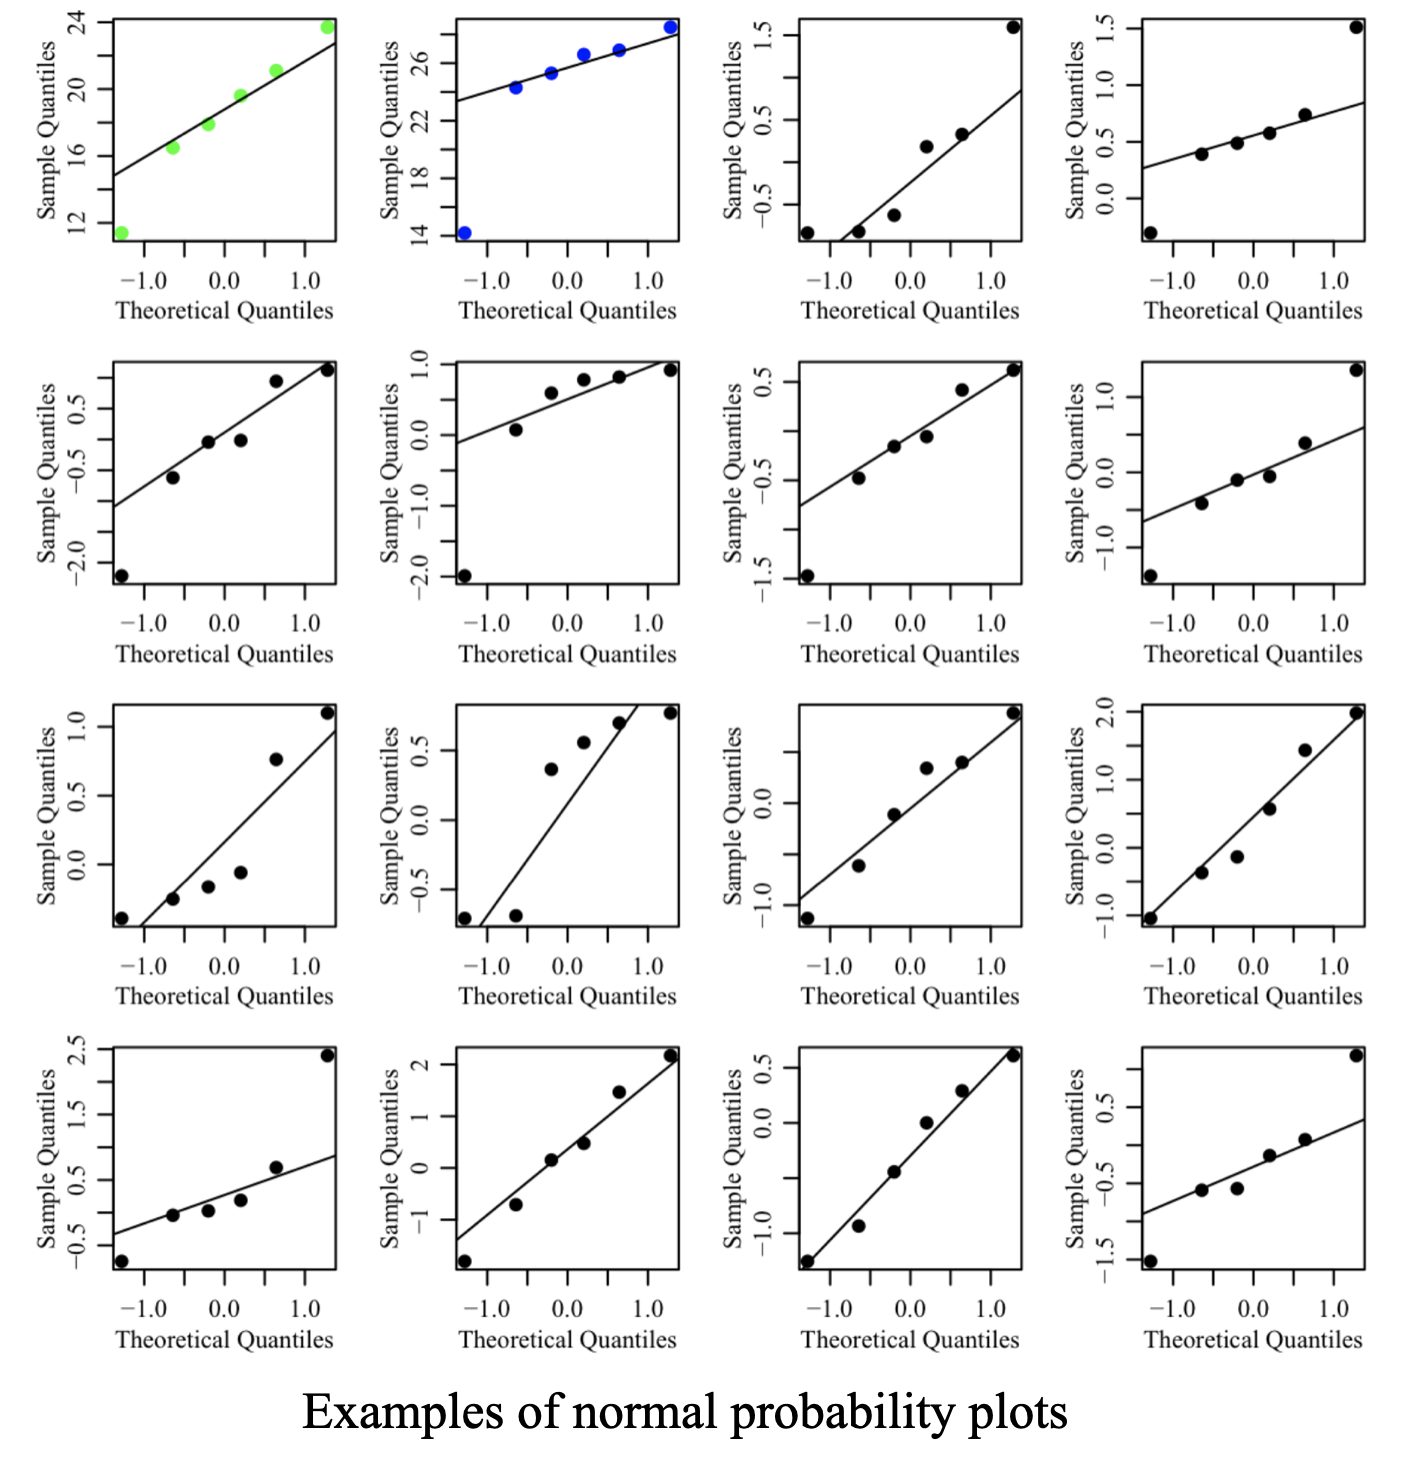
\includegraphics[width=1\textwidth]{fig19.png}
\end{figure}

\newpage
\section*{Checking Equality of Variances}

There is a formal procedure (e.g., Levene's test). We will see this later.

\noindent For now, we can use the following rule of thumb:

\[
\frac{1}{4} < \frac{S_A^2}{S_B^2} < 4 \quad \textcolor{red}{\text{(A, B can reverse)}}
\]

\noindent \textbf{What if variances do not appear to be equal?}

Options:
\begin{enumerate}
    \item Use randomization $H_0$ distribution.
    \item Transform data to stabilize variances.
    \item Use modified t-test that allows unequal variances:
\end{enumerate}

\[
\textcolor{blue}{t_W(Y_A, Y_B) = \frac{\overline{Y}_B - \overline{Y}_A}{\sqrt{\frac{S_A^2}{n_A} + \frac{S_B^2}{n_B}}}}
\]
\[
\textcolor{red}{\text{W: df based on Welch's approximation}}
\]

\section*{Example: Two-Sample t-test}

\begin{itemize}
    \item Compare the effects of two soporific drugs
    \begin{itemize}
        \item Optical isomers of hyoscyamine hydrobromide
    \end{itemize}
    
    \item Each subject receives a placebo and then is randomly assigned to receive Drug 1 or Drug 2
    
    \item Dependent variable: Number of hours of increased sleep over control
    
    \item Drug 1 given to $n_1$ subjects, Drug 2 given to $n_2$ different subjects
    
    \item Study question: Is Drug 1 or Drug 2 more effective at increasing sleep?
    \begin{itemize}
        \item $H_0: \mu_1 = \mu_2$
        \item $H_1: \mu_1 \neq \mu_2$
    \end{itemize}
\end{itemize}

\begin{center}
\begin{tabular}{ c c c }
\hline
\textbf{Obs.} & \textbf{Drug 1} & \textbf{Drug 2} \\
\hline
1  & 0.7  & 1.9 \\
2  & -1.6 & 0.8 \\
3  & -0.2 & 1.1 \\
4  & -1.2 & 0.1 \\
5  & -0.1 & -0.1 \\
6  & 3.4  & 4.4 \\
7  & 3.7  & 5.5 \\
8  & 0.8  & 1.6 \\
9  & 0.0  & 4.6 \\
10 & 2.0  & 3.4 \\
\hline
\textbf{Mean} & 0.75 & 2.33 \\
\textbf{SD}   & 1.79 & 2.0 \\
\hline
\end{tabular}
\end{center}

\begin{figure}[H]
    \centering
    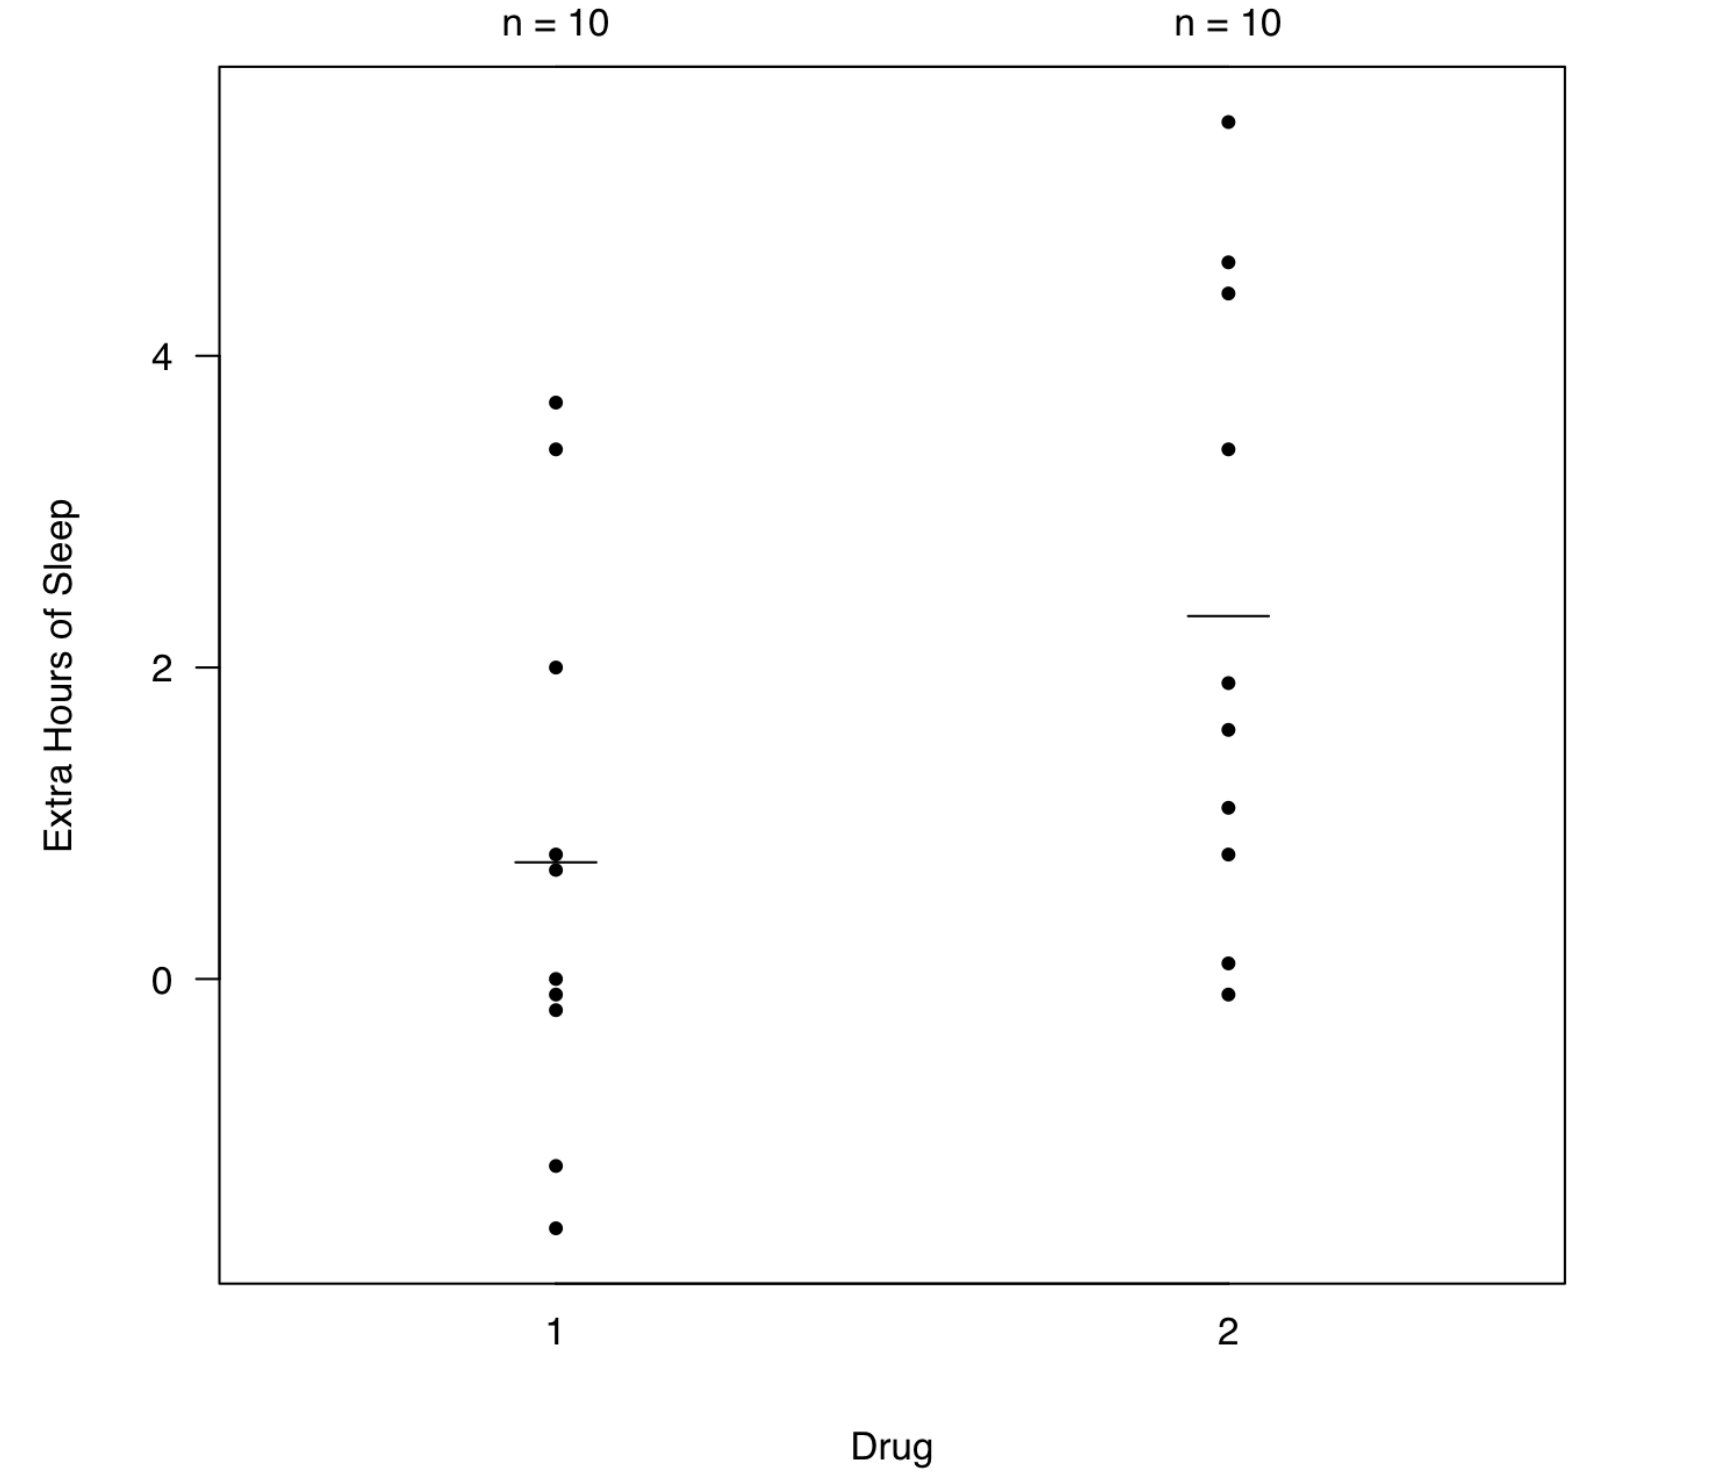
\includegraphics[width=1\textwidth]{fig20.png}
\end{figure}

\begin{figure}[H]
    \centering
    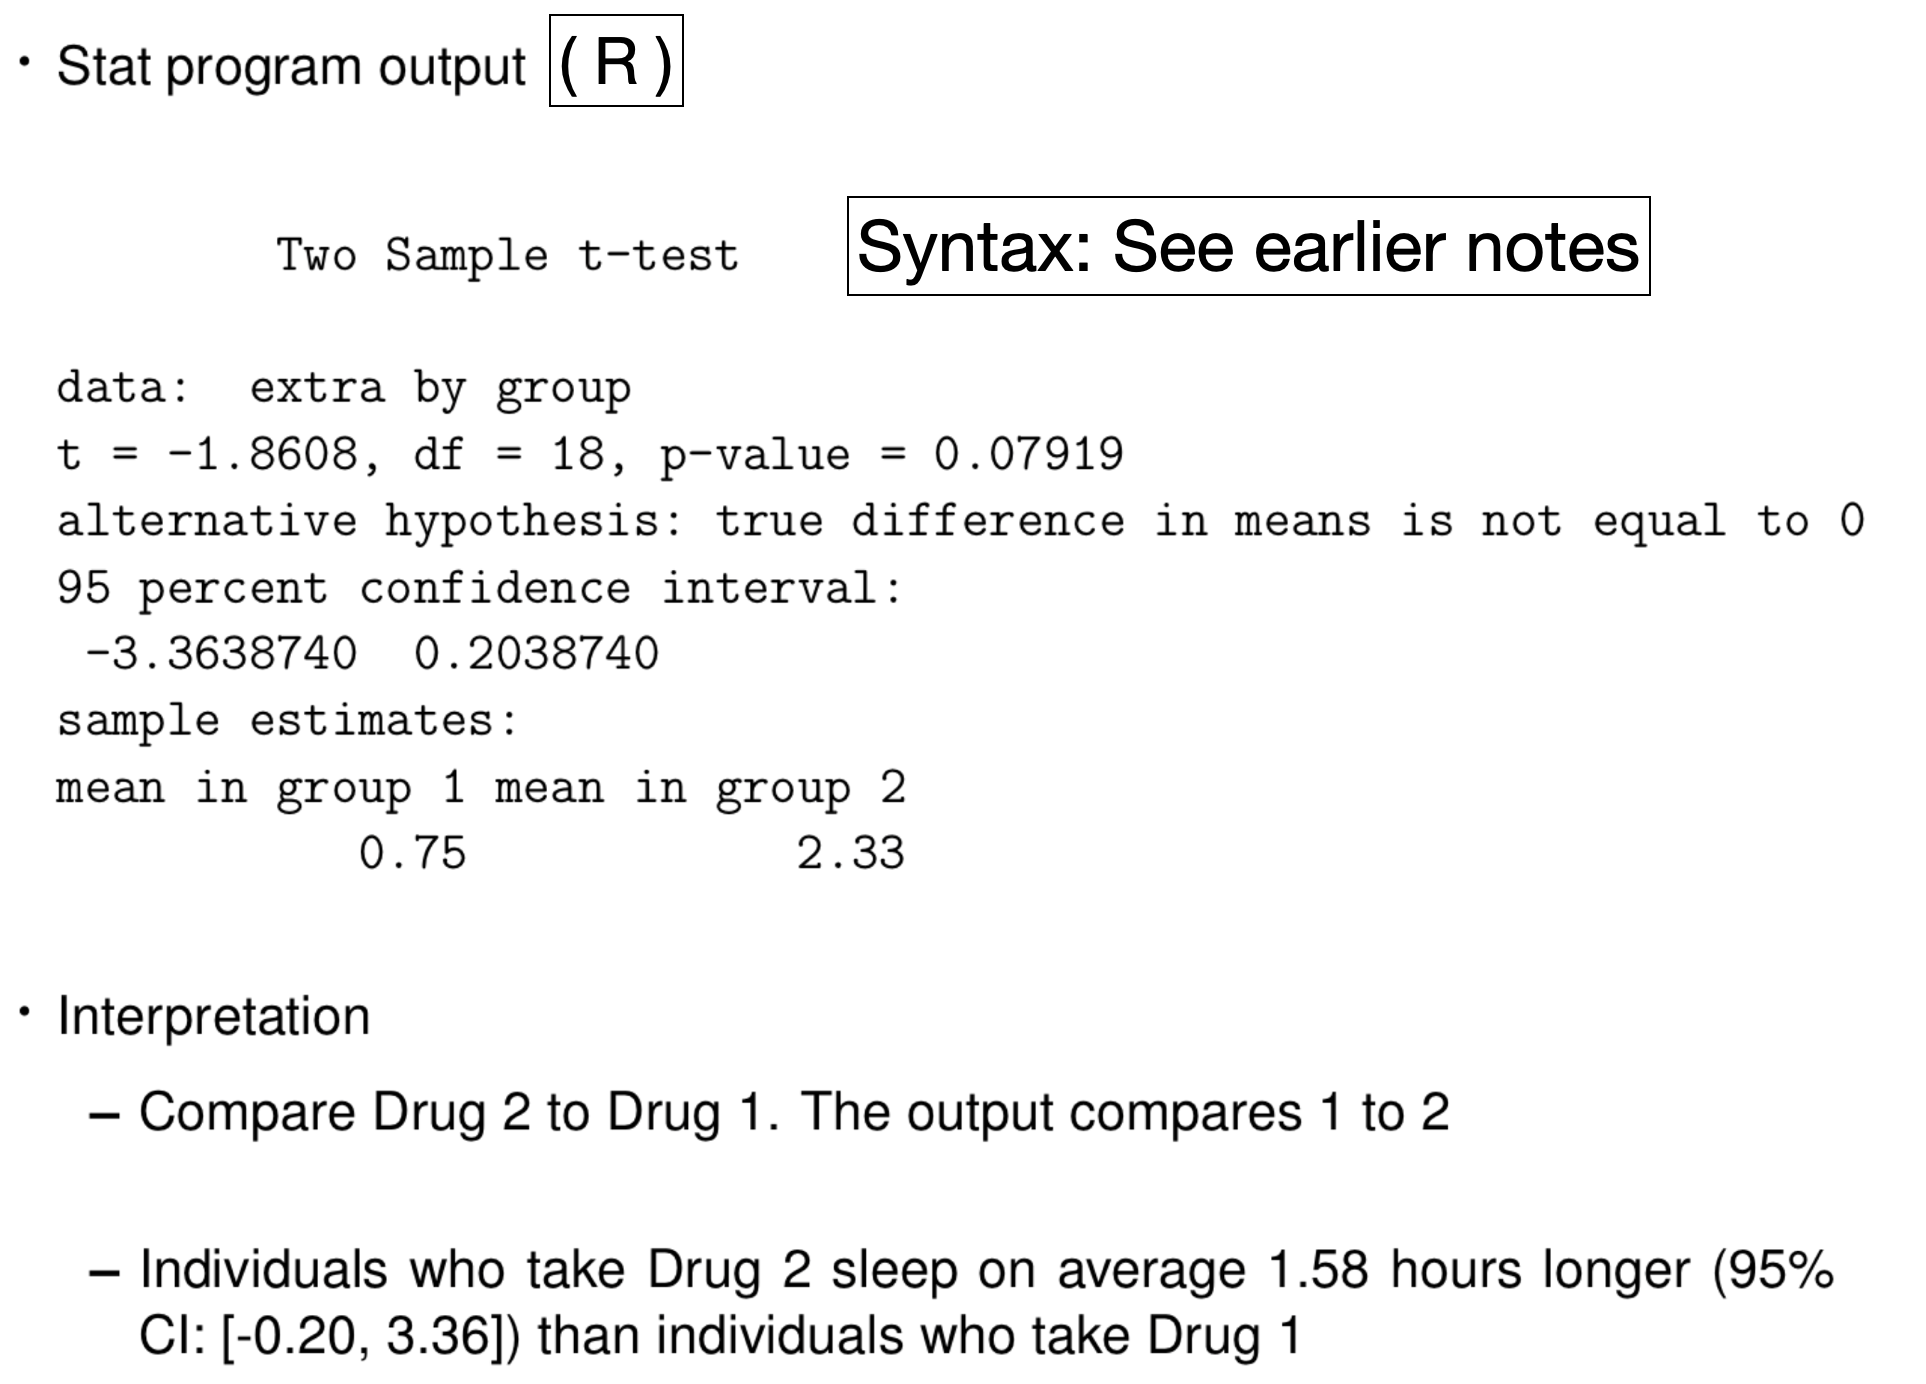
\includegraphics[width=1\textwidth]{fig21.png}
\end{figure}

\begin{figure}[H]
    \centering
    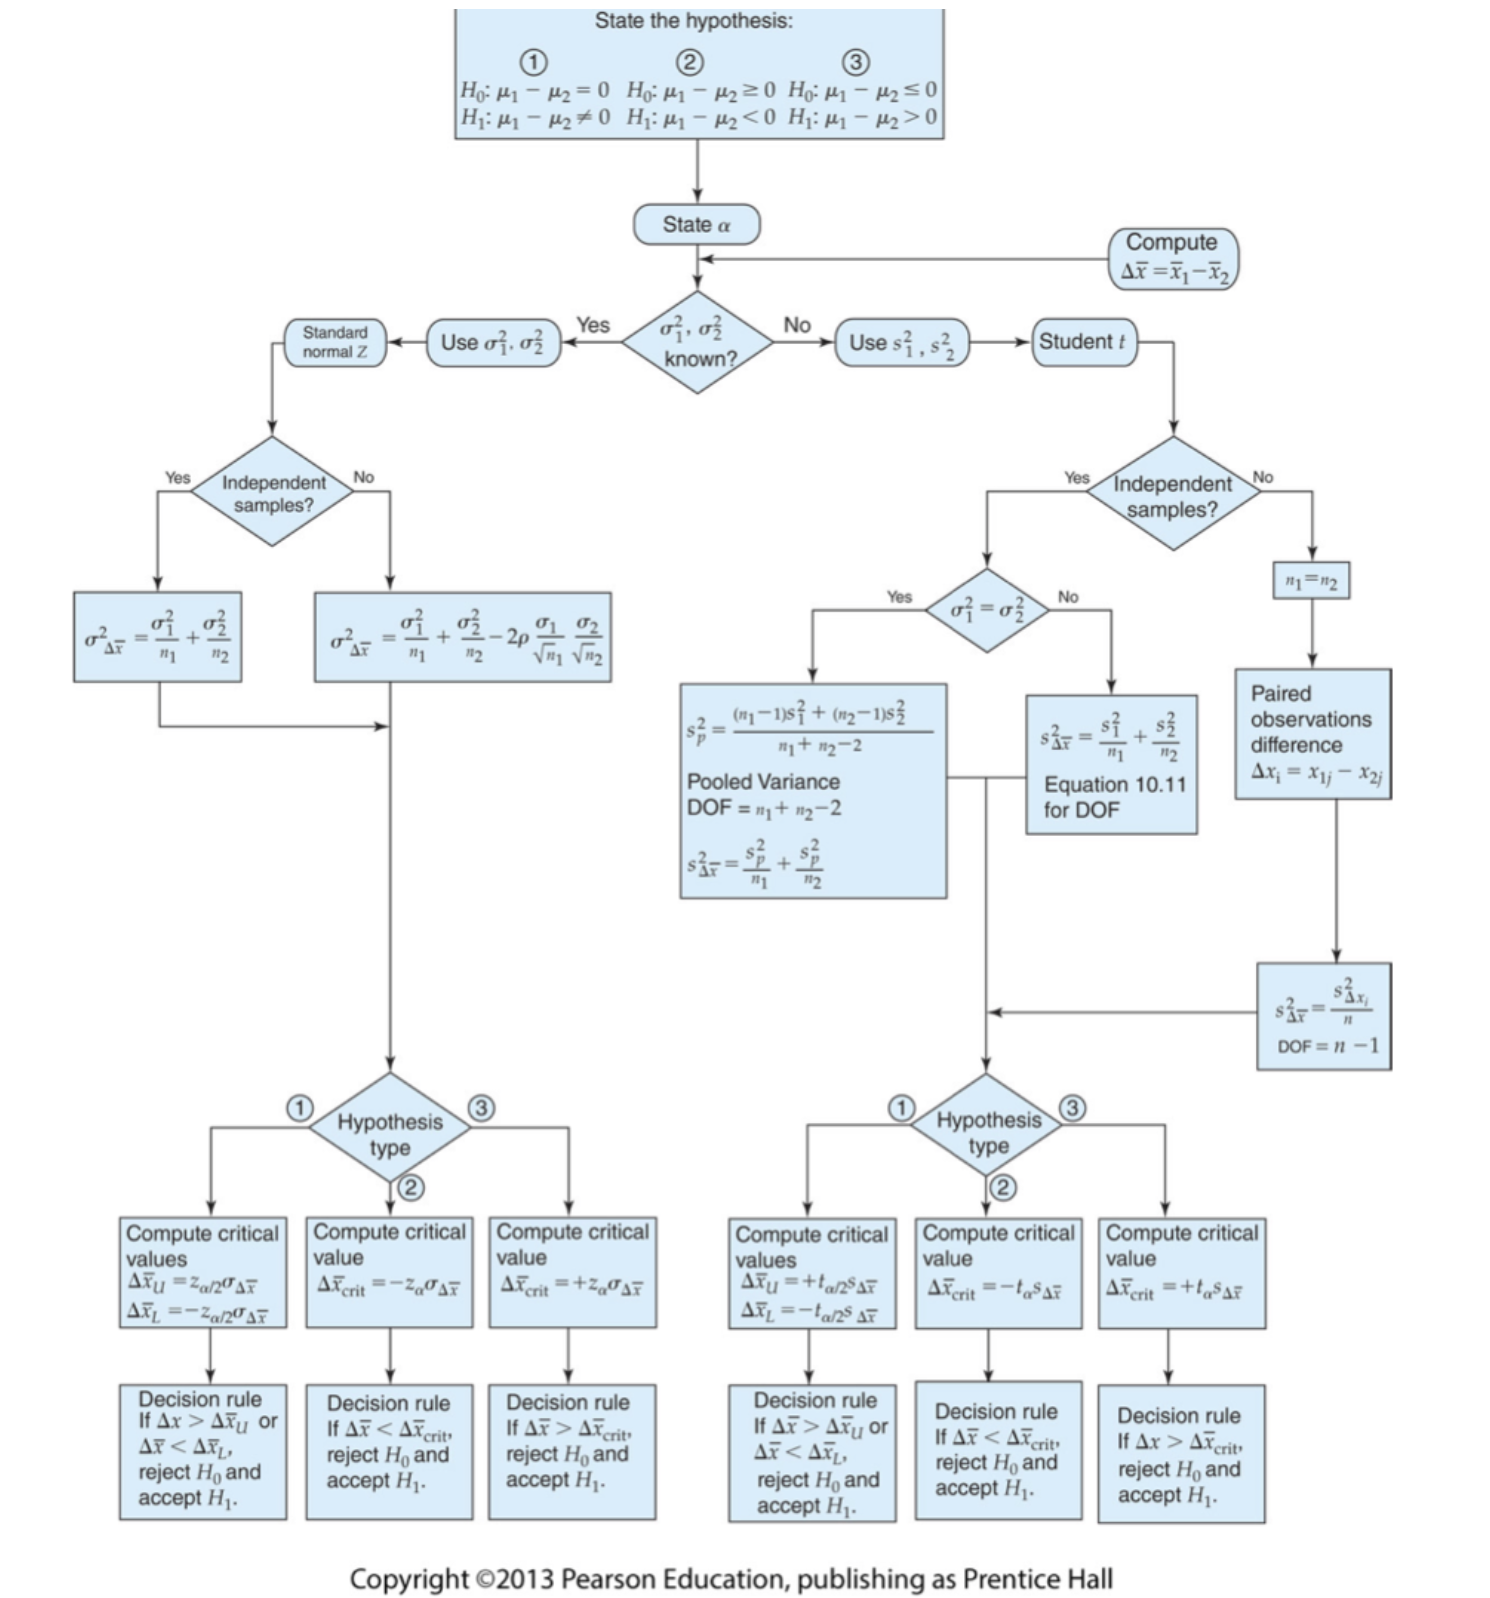
\includegraphics[width=1\textwidth]{fig22.png}
\end{figure}

\begin{figure}[H]
    \centering
    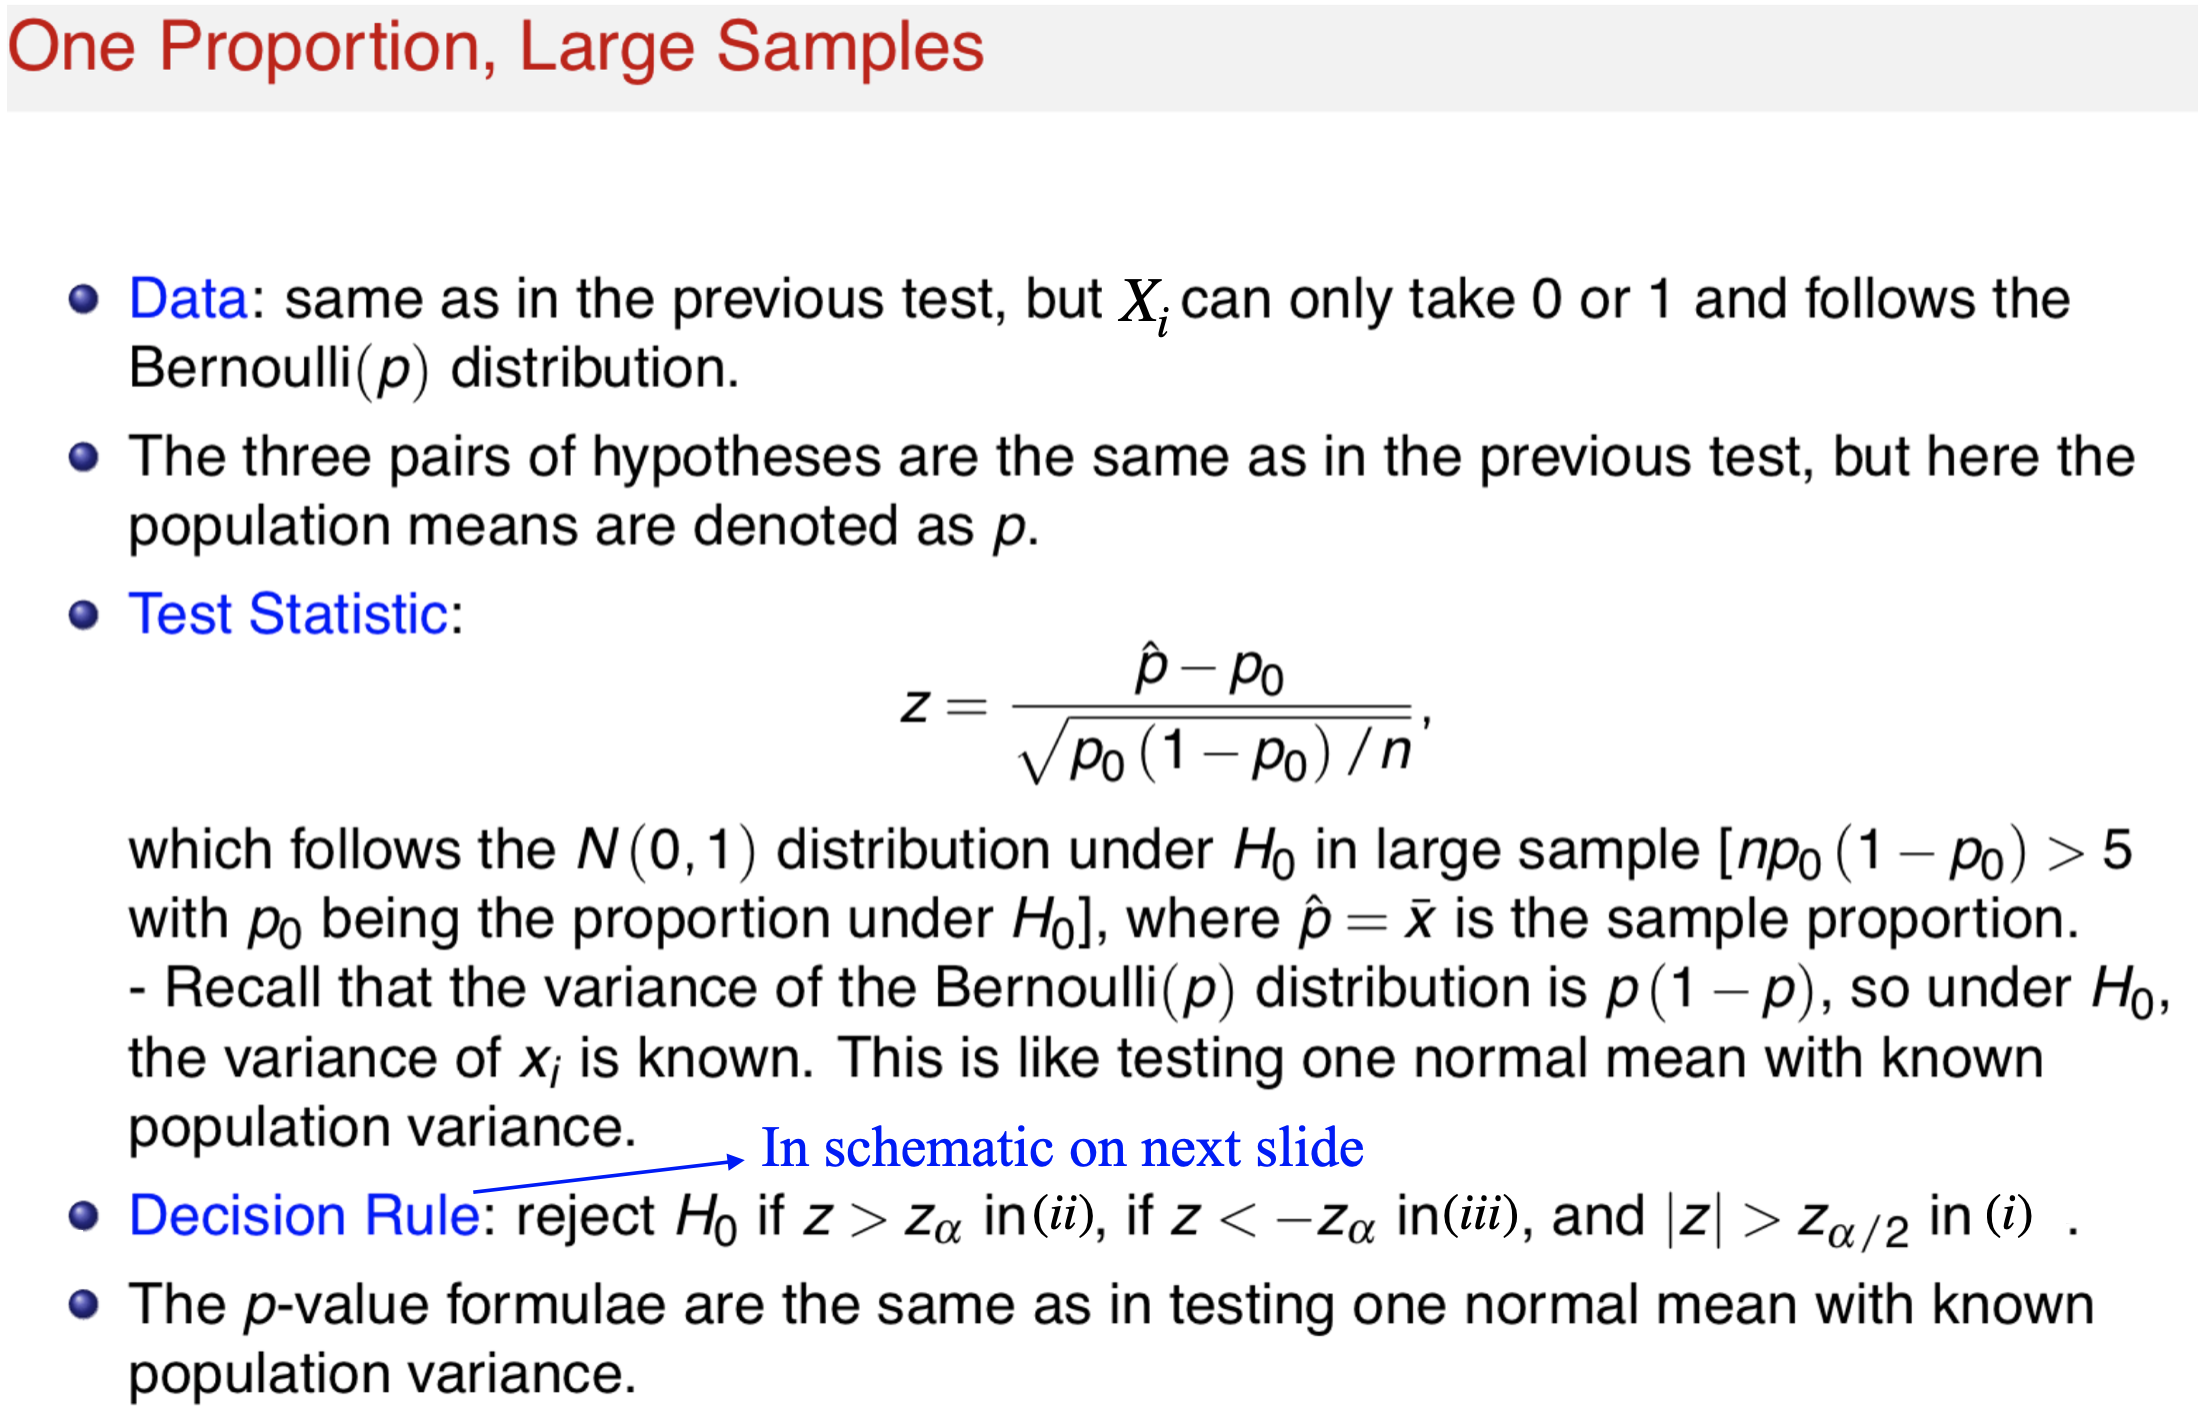
\includegraphics[width=1\textwidth]{fig23.png}
\end{figure}

\begin{figure}[H]
    \centering
    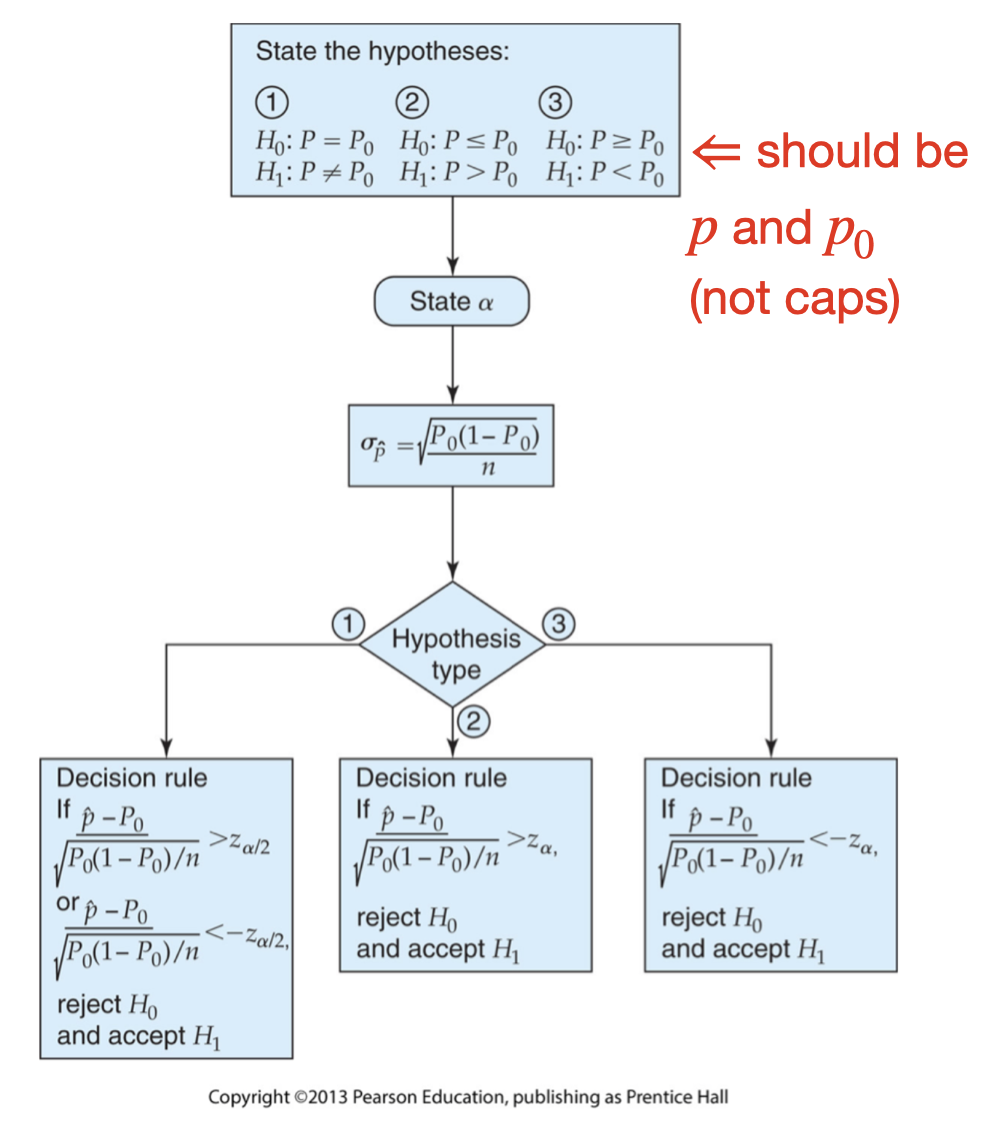
\includegraphics[width=1\textwidth]{fig24.png}
\end{figure}

\begin{figure}[H]
    \centering
    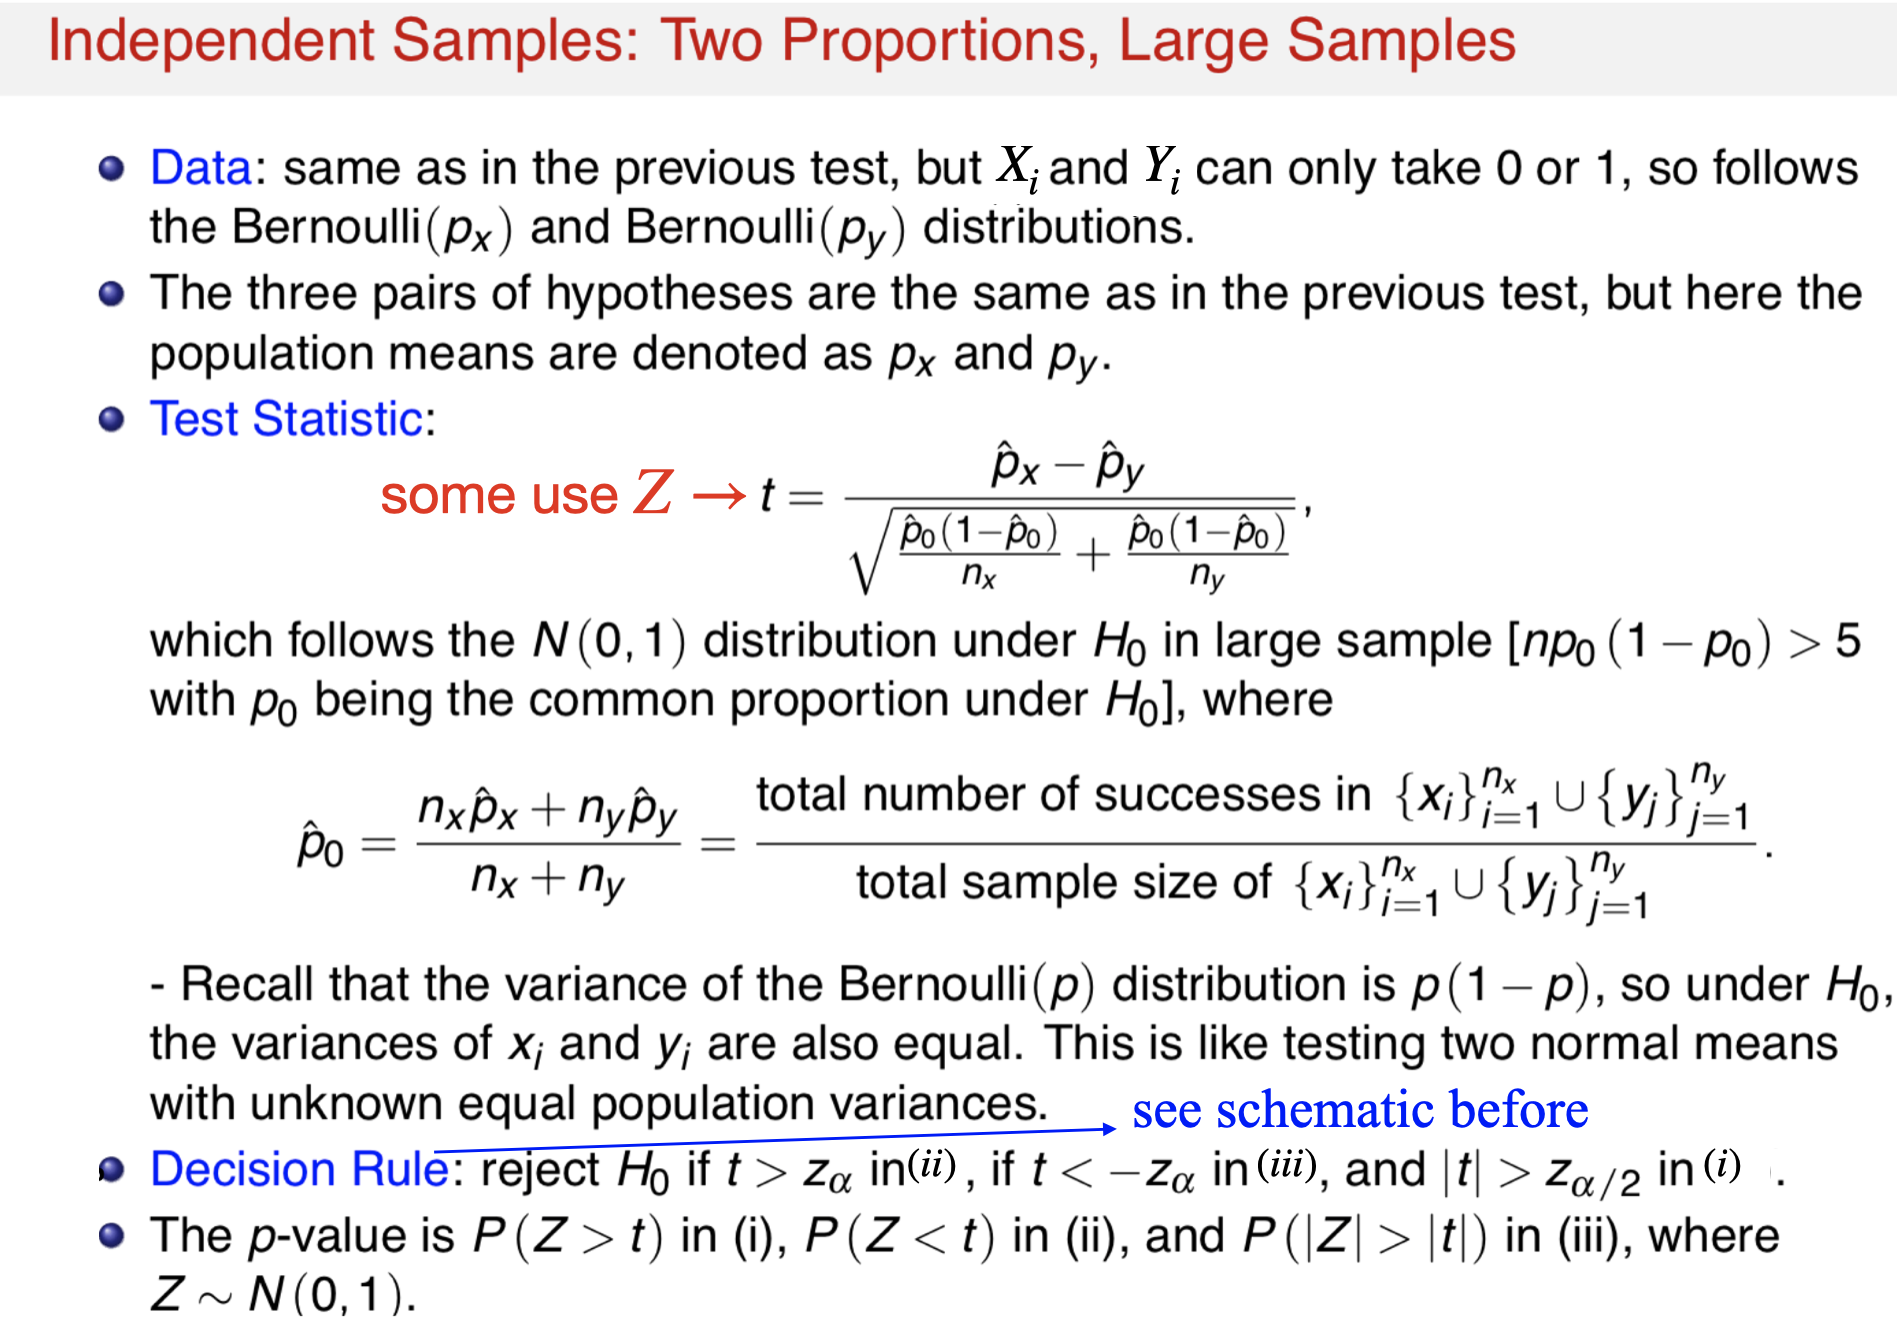
\includegraphics[width=1\textwidth]{fig25.png}
\end{figure}

\begin{figure}[H]
    \centering
    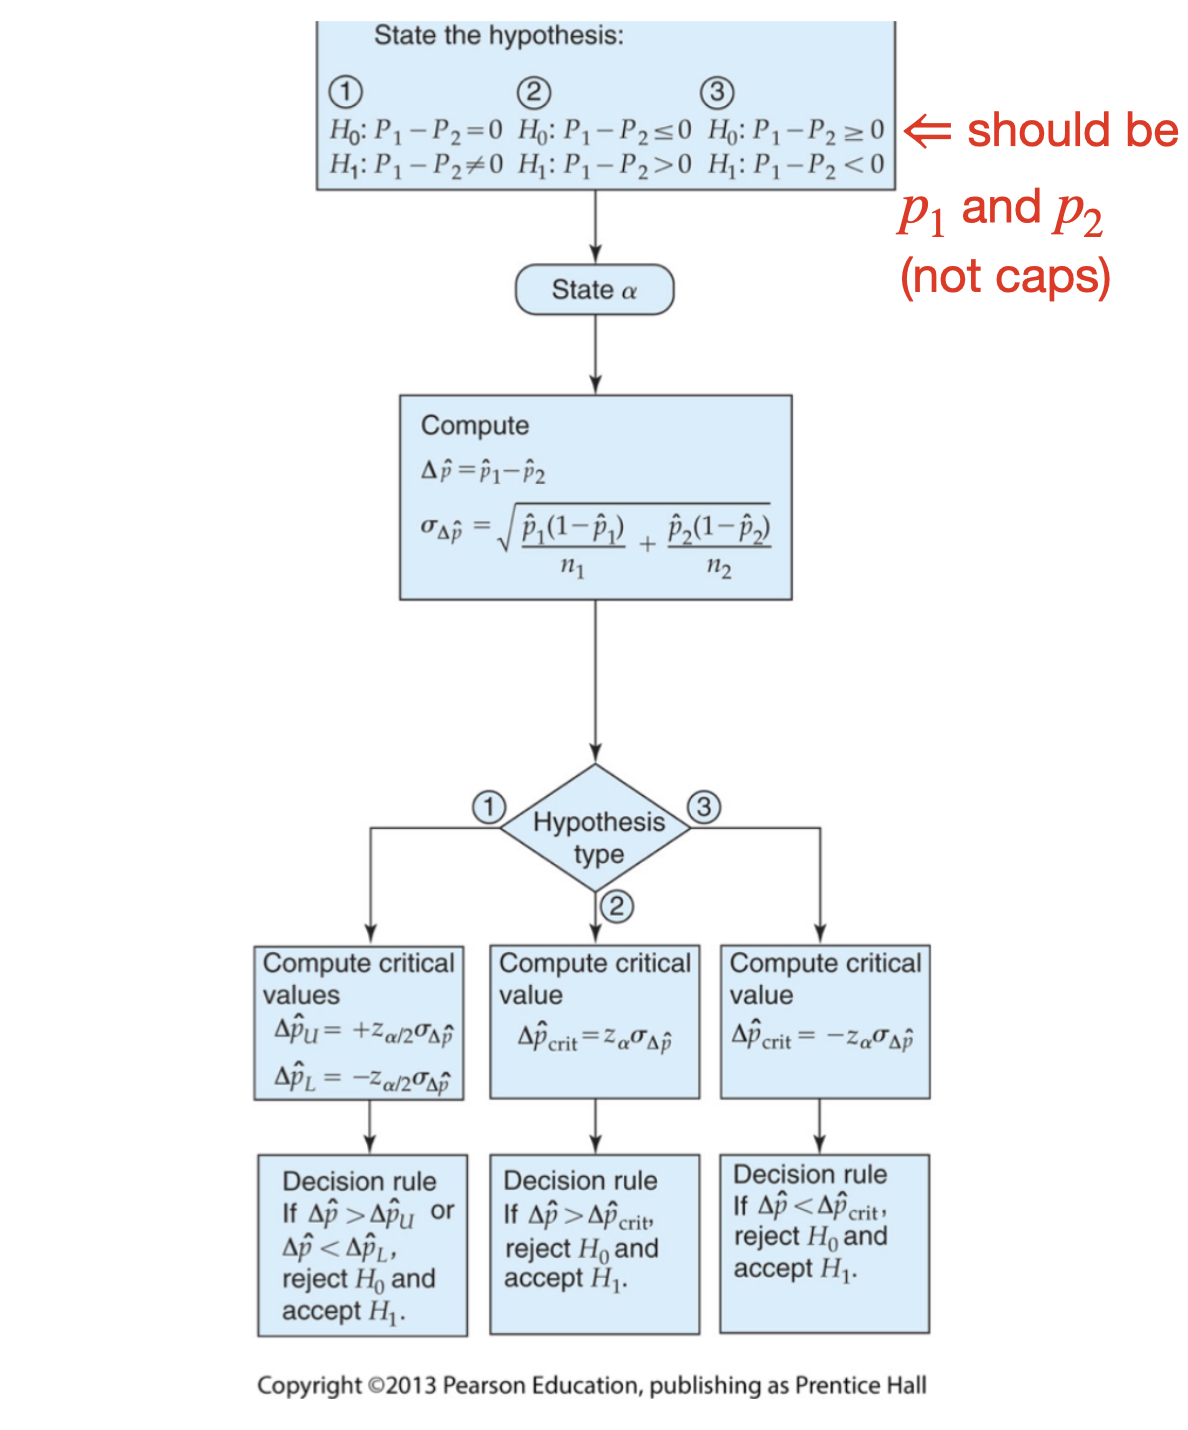
\includegraphics[width=1\textwidth]{fig26.png}
\end{figure}

\newpage

\noindent
\textbf{Example:} \\
Test whether the population of women whose age at first birth $\leq 29$ has the same probability of breast cancer as women whose age at first birth was $\geq 30$. This dichotomization is highly arbitrary and we should really be testing for an association between age and cancer incidence, treating age as a continuous variable.

\begin{itemize}
    \item \textbf{Case-control study} (independent and dependent variables interchanged); $p_1 = $ probability of age at first birth $\geq 30$, etc.
    
    \begin{center}
    \begin{tabular}{|l|c|c|}
    \hline
    & \textbf{with Cancer} & \textbf{without Cancer} \\
    \hline
    Total \# of subjects & 3220 ($n_1$) & 10245 ($n_2$) \\
    \# age $\geq$ 30     & 683  & 1498 \\
    \hline
    Sample probabilities & 0.212 ($\hat{p}_1$) & 0.146 ($\hat{p}_2$) \\
    \hline
    \end{tabular}
    \end{center}
    
    \begin{itemize}
        \item Pooled probability:
        \[
        \frac{683 + 1498}{3220 + 10245} = 0.162
        \]
    \end{itemize}

    \item \textbf{Estimate the variance}
    \[
    \text{variance}(\hat{p}_1 - \hat{p}_2) = \hat{p_0}(1 - \hat{p_0}) \times \left[ \frac{1}{n_1} + \frac{1}{n_2} \right] = 5.54 \times 10^{-5}
    \]
    \[
    SE = \sqrt{\text{variance}} = 0.00744
    \]
    
    \item \textbf{Test statistic}
    \[
    z = \frac{0.212 - 0.146}{0.00744} = 8.85
    \]
    
    \item 2-tailed $P$-value is 0.0 using \texttt{survstat}; we report $P < 0.0001$

    \item We do not use a $t$-distribution because there is no $\sigma$ to estimate (and hence no "denominator d.f." to subtract).
\end{itemize}


\section*{Other testing approaches include:}

\begin{itemize}
    \item $\chi^2$ test
    \item Fisher's exact test
\end{itemize}












\end{document}
